% This is samplepaper.tex, a sample chapter demonstrating the
% LLNCS macro package for Springer Computer Science proceedings;
% Version 2.20 of 2017/10/04
%
\documentclass[runningheads]{llncs}
%
\usepackage{graphicx}
\usepackage[portuges]{babel}
\usepackage[T1]{fontenc}
\usepackage{verbatim}
\usepackage{float}
%Path relative to the .tex file containing the \includegraphics command
\graphicspath{ {./images/} }
% Used for displaying a sample figure. If possible, figure files should
% be included in EPS format.
%
% If you use the hyperref package, please uncomment the following line
% to display URLs in blue roman font according to Springer's eBook style:
% \renewcommand\UrlFont{\color{blue}\rmfamily}
\setcounter{secnumdepth}{6}
\renewcommand\theparagraph{\Alph{paragraph}}
 
\makeatletter
\renewcommand\paragraph{\@startsection{paragraph}{4}{\z@}%
                                      {-3.25ex\@plus -1ex \@minus -.2ex}%
                                      {0.0001pt \@plus .2ex}%
                                      {\normalfont\normalsize\bfseries}}
\renewcommand\subparagraph{\@startsection{subparagraph}{5}{\z@}%
                                      {-3.25ex\@plus -1ex \@minus -.2ex}%
                                      {0.0001pt \@plus .2ex}%
                                      {\normalfont\normalsize\bfseries}}
 
\counterwithin{paragraph}{subsubsection}
\counterwithin{subparagraph}{paragraph}
\makeatother

\begin{document}
%
\title{MSTG - Teste de aplicações Android e iOS}
%
%\titlerunning{Abbreviated paper title}
% If the paper title is too long for the running head, you can set
% an abbreviated paper title here
%
%\author{Adriana Lopes \and Diana Carrilho \and Henrique Faria \and Paulo Barbosa}
\author{}
%
% First names are abbreviated in the running head.
% If there are more than two authors, 'et al.' is used.
%
\institute{Departamento de Informática, Universidade do Minho}
%
\maketitle              % typeset the header of the contribution
%
% Abstract
\begin{abstract}

\keywords{MSTG  \and Android \and iOS.}
\end{abstract}
%
%
% Introdução
\begin{center}
\normalsize{\bfseries Introdução}\hfill 
\end{center}








\newpage
\hfill
% Aqui começam os capitulos abordados pelo trabalho
\section{OWASP ZAP}

\subsection{OWASP-ZAP Layout}

Nesta secção pretendemos explicar todos os recursos importantes disponibilizados pelo ZAP. E a configuração da interface do mesmo.


\subsubsection{Desktop UI Overview}

\paragraph{Top Level Menu}

Em primeiro lugar vamos referir as opções oferecidas pelo menu superior da aplicação. Este menu oferece acesso a praticamente todos os recursos do ZAP e não só isso como também permite configurar os mesmos.

\begin{itemize}
\item File menu\newline

\par Permite que possamos criar uma nova sessão, importar uma sessão guardada, apagar a sessão atual, guarda-la ou sair da aplicação.

\item Edit menu \newline

\par Permite mudar o modo em que o ZAP opera: 

- safe: não são realizadas operações potencialmente perigosas.

- protected: só podemos realizar operações potencialmente perigosas nos URLs especificados

- Standard: podemos realizar qualquer operação que o ZAP suporte

- ATTACK: novos nodos que entram na "mapa" resultados do spider do site são ativamente scaneados mal seja descobertos.

\par Permite manter o utilizador autenticado no site alvo com a opção \textit{forced user mode}.


\item View menu \newline

\par Permite ver a \textit{history tab}, que por sua vez mostra todos os pedidos feitos ordenados no tempo possuindo as informações de index, método HTML usado (GET/POST), URL, código de resposta HTTP, explicação do que significa o código anterior, o tempo que demorou o pedido, qualquer alerta de vulnerabilidade no pedido, notas adicionadas ao pedido e tags associadas ao mesmo.  


\item Analyse menu \newline

\par Este menu permite modificar uma politica de análise\footnote[1]{Uma politica de análise define um conjunto de regras a serem seguidas durante uma análise átiva. Também define quants pedidos são feitos e quão provável será potenciais problemas serem assinalados.} ou adicionar uma nova.


\item Report menu  \newline

\par permite gerar um relatórico com todos os alertas encontrados em formato HTML, XML ou Markdown.

\item Tools menu \newline

\par Este menu pemite aceder ás opções de configuração das ferramentas e recursos disponíveis no ZAP.
\begin{itemize}
\item Nas configurações de scan ativo podemos definir:\newline

\par - O número de hosts a serem analisados ao mesmo tempo;\newline

\par - Quantas threads existirão por host;\newline

\par - O nnúmero de resultados que aparecerão na tab do scan ativo;\newline

\par - O tempo máximo que uma regra da politica de análise poderá demorar;\newline

\par - O tempo máximo que um scan pode demorar;\newline

\par - O delay em (milisegundos) entre pedidos feitos;\newline

\par - Se queremos que seja injetado em cada pedido o identificador do mesmo no ZAP na forma X-ZAP-Scan-ID;\newline

\par - Se queremos que durante o scan o zap tente obter tokens anti CSRF\footnote[2]{OS tokens Anti CSRF são parâmetros pseudo aleatórios usados para proteção contra ataques de Cross Site Request Forgery (CSRF).};\newline

\par - Usar a definição padrão de análise ativa;\newline

\par - Usar a definição padrão de análise de ataque; \newline


\item Nos vetores de input do scan ativo podemos definir como inputs:

\par - Strings de URL específicas após o ?; \newline

\par - Pares chave-valor nos dados Post pedidos; \newline

\par - Elementos de caminhos URL; \newline

\par - Cabeçalhos HTTP; \newline

\par - Cookies; \newline

\item Podemos adicionalmente escolher o formato dos inputs do scan ativo sendo estes:

\begin{itemize}

\item Multipart Form Data	
\item XML tag/attribute	
\item JSON	
\item Google Web Toolkit	
\item OData id/filter

\end{itemize}

\item Podemos definir como queremos que os alertas nos sejam apresentados:

\par - Podemos reduzir o tamanho dos relatórios significativamente caso façamos merge de alertas iguais encontrados em pontos diferentes do scan.  \newline
\par - Podemos também escolher o número máximo de alertas que pretendemos que constem no relatório. \newline
\par - Por último é-nos dada a opão de modificar a mensagem associada com um alerta específico para melhor compreensão. \newline

\item Outro ponto configurável são os tokens anti CRSF, podemos escolher quais queremos analisar.

\item Podemos definir o endereço e a porta em que o ZAP vai ficar á escuta de conecções, caso não sejam definidos o ZAP usa o localhost como endereço e liga-se a uma porta aleatória disponível na máquina. 

\item O ZAP permite gerar um certificado SSL dinâmico para os casos em que as aplicações usem SSL mútuo.\newline
\par Para permitir conecções SSL trasparentes é necessário encriptar cada pedido feito ao servidor e desencriptar cada reposta do mesmo, como o browser usado já faz isso, a única maneira de o ZAP fazer isto é atrvés de um ataque "man-in-the-middle". Para isto basta que adicionemos aos certificados de confiança do browser escolhido o ZAP Root CA certificate. Desta forma como o ZAP cria um certificado assinado para cada servidor sobre o qual realiza o ataque "man-in-the-middle", usar o ZAP Root CA certificate é uma forma de assegurar ao browser que pode confiar nesse certificado.

\item O ZAP também permite definir e configurar o tipo de conecção a ser usada:

\par - Podemos definir um timeout que o que facilita o teste de aplicações lentas.\newline
\par - Podemos definir o utilizador que o ZAP deve sar ao criar asa mensagens HTTP.\newline
\par - Podemos definir se o ZAP usa um "Single cookie request header" ou "multiple cookie request header"\footnote[3]{O Cookie HTTP request header contem cookies HTTP enviadas previamente em respostas do servidor, o Zap possibilita enviar as cookies todas juntas ou uma de cada vez por HTTP request header.}.\newline
\par - Podemos ativar o (Global) HTTP State, isto é, podemos rastrear as cookies guardadas na sessão.\newline
\par - Podemos definir por quanto tempo as queries DNS bem sucedidas devem ser guardadas em cache (números negativos represetam sem limite de tempo, zero não permite guardar e números positivos representam o tempo em segundos a guardar).\newline
\par - Podemos ainda definir as versões dos protocolos a usar nas conecções efetuadas. Devemos no entanto ter a opção "SSLv2Hello" selecionadacom pelo menos uma versão de SSL/TLS. \newline


\item Podemos também definir vários regex para URLs que o ZAP irá ignorar. Estes regex podem ser ainda modificados ou removidos.
\end{itemize}

\item Help menu \newline


\par - Neste menu podemos procurar ajuda sobre como utilizar o ZAP, procurar ajuda para resolver problemas de versões do ZAP e add-ons e para verificar a existencia de updates.\newline

\end{itemize}

\paragraph{Toolbar Menu} \hfill\newline
\hfill\newline
\par Neste menu podemos encontrar formas de dispor o layout do ZAP para que se torne mais agradável á vista ou para podermos visualizar vários paineis úteis simultaneamente. Neste menu destacam-se algumas features que achamos interessantes nomeadamente:\newline

\begin{figure}[H]

  \centering

  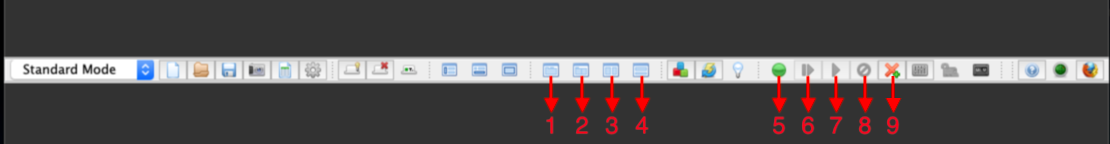
\includegraphics[scale = 0.31]{fig18.png}

  \caption{Toolbar Menu}

\end{figure}

\par Neste menu podemos definir se queremos colocar os pedidos feitos ao servidor e as respetivas respostas ao servidor lado a lado. Para isso temos 2 opções disponíveis.


\begin{enumerate}

\item Colocar os pedidos e respostas em tabs lado a lado.
\item Colocar os pedidos e respostas na mesma tab lado a lado.
\item Colocar os pedidos na parte esquerda de uma tab e as respetivas respostas na direita.
\item Colocar os pedidos na parte superior de uma tab e as respetivas respostas na inferior.

\par Adicionalmente este menu permite um controlo maior sobre os pedidos e as respostas do servidor, permitindo-nos adicionar um break em cada pedido, resposta ou nos dois e modificar os pedidos, evitar que um pedido seja feito ou remover um par pedido-resposta. O botão usado para implementar os breaks é  o circulo assinalado pelo número 5.\newline

\par Possuimos também auxiliares para trabalhar com os breakpoints assinalados com os números 6,7,e 8 que executam as seguintes ações sobre os pedidos e respostas apanhadas respetivamente saltar para o próximo par pedido resposta, continuar a realizar os pedidos e respostas e parar apenas no caso de termos definido um breakpoint para um URL específico\footnote[4]{Um breakpoint pode ser definido para um URL especifico com recurso ao elemento identifocado como 9.} e destruir o par pedido-resposta apanhado pelo breakpoint. \newline
\end{enumerate}

\paragraph{Windows} \hfill\newline
\hfill\newline
\begin{enumerate}

\item Sites Window, nesta podemos ver toda a informação referente aos sites que visitamos, isto inclui o URL, pedidos GET associados ao URL, pastas ocultas encontradas neste entre outros.

\begin{figure}[H]

  \centering

  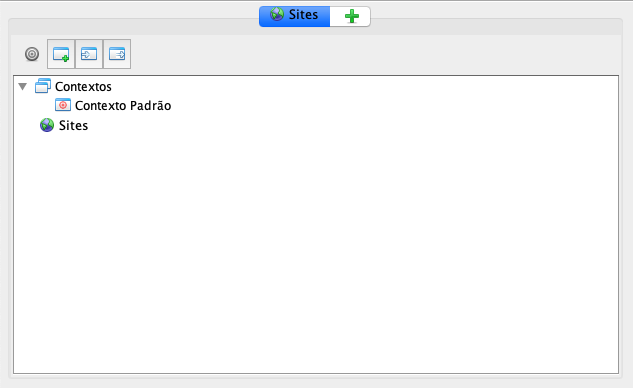
\includegraphics[scale = 0.31]{fig19.png}

  \caption{Sites Window}

\end{figure}

\item Workspace Window, nesta podemos visualizar as informações dos pedidos e as respetivas respostas. Também é nesta janela que podemos efetuar alterações aos mesmos quando temos breakpoints definidos.

\begin{figure}[H]

  \centering

  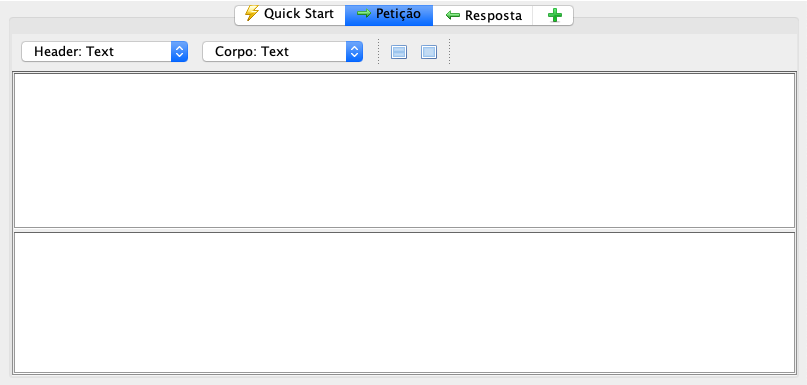
\includegraphics[scale = 0.31]{fig20.png}

  \caption{Workspace Window}

\end{figure}

\item Information Window, nesta última janela encontramos todas as informações úteis referentes aos testes de segurança realizados sobre um site. As informações estão organizadas nas seguintes tabs:
\begin{itemize}
	\item History tab: Mostra os pedidos pela ordem em que foram feitos, permitindo modificar a ordem pelo atributo que o utilizador quiser (url, método, código, alerta mais importante,...).
	\item Search tab: Permite uma pesquisa entre todos os pedidos e respostas de um teste.

	\item Breakpoints tab: mostra os breakpoints feitos num teste.

	\item Alerts tab: Mostra todos os alertas encontrados na aplicação durante o teste.

	\item Active Scan tab: Mostra os scans ativos 

	\item Spider tab: Mostra os URLs que ainda não foram visitados

	\item Params tab: Mostra um sumário dos parâmetros que um site utiliza.

	\item Output tab: Mostra várias mensagens informativas sobre o teste realizado.

	\item Callbacks tab: Mostra pedidos de callbacks que o ZAP recebeu durante os testes ao site.

\end{itemize}
\begin{figure}[H]

  \centering

  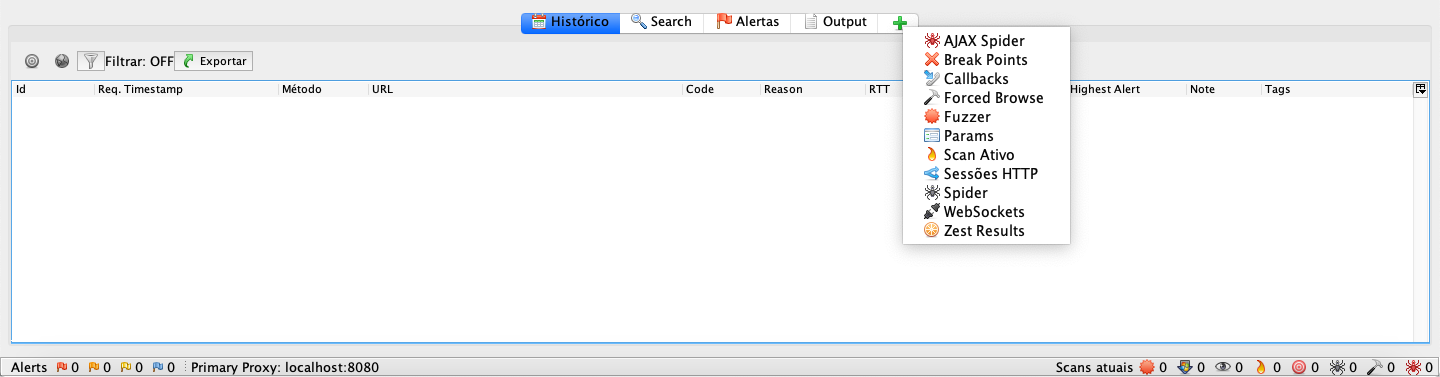
\includegraphics[scale = 0.31]{fig21.png}

  \caption{Information Window}

\end{figure}
\end{enumerate}



\subsection{Preparação dos recursos}

Agora que já sabemos mexer no ZAP temos de começar por preparar o site sobre o qual vamos efetuar os nossos testes. Para este site usaremos o mutillidae configurando o Metasploitable para o correr e o Firefox para podermos aceder ao mesmo.

\subsubsection{Metasploitable}

 configurar o ficheiro config.inc:

  \$dbname = 'metasploit' -> \$dbname = 'owasp10'
\begin{figure}[H]

  \centering

  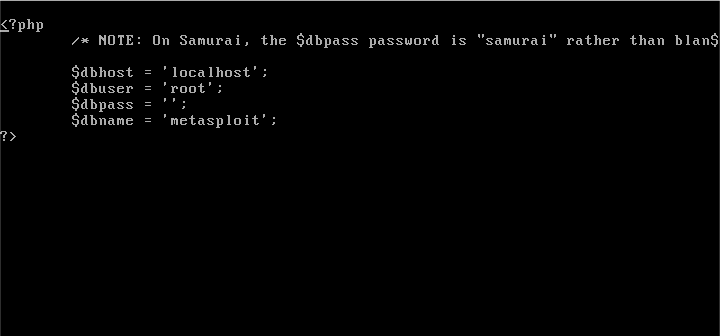
\includegraphics[scale = 0.31]{fig1.png}

  \caption{Antes da configuração do ficheiro config.inc}

\end{figure}

\begin{figure}[H]

  \centering

  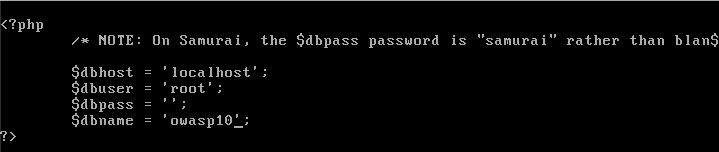
\includegraphics[scale = 0.31]{fig2.png}

  \caption{ficheiro config.inc corretamente configurado}

\end{figure}


De seguida temos de ir a etc/php5/cgi e configurar o ficheiro \textit{php.ini}.
Neste fichero temos primeiro de encontrar os fopen wrappers corretos, para isso podemos usar o comando "ctr + w" para procurar "fopen". Agora basta-nos modificar a opção allow\_url\_include = Off para allow\_url\_include = On, como se vê nas figuras seguintes.

\begin{figure}[H]

  \centering

  
\includegraphics[scale = 0.31]{fig3.png}
 
  \caption{Opção a encontrar para ser modificada}

\end{figure}

\begin{figure}[H]

  \centering

  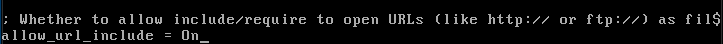
\includegraphics[scale = 0.31]{fig4.png}

  \caption{Opção modificada}

\end{figure}

Agora só precisamos de reiniciar o servidor. A figura seguinte mostra o comando usado para reiniciar o servidor apache : \textit{"sudo /etc/init.d/apache2 restart"} e o comando ifconfig para visualizarmos o endereço IP da Máquina virtual para posterior utilização no Firefox.

\begin{figure}[H]

  \centering

  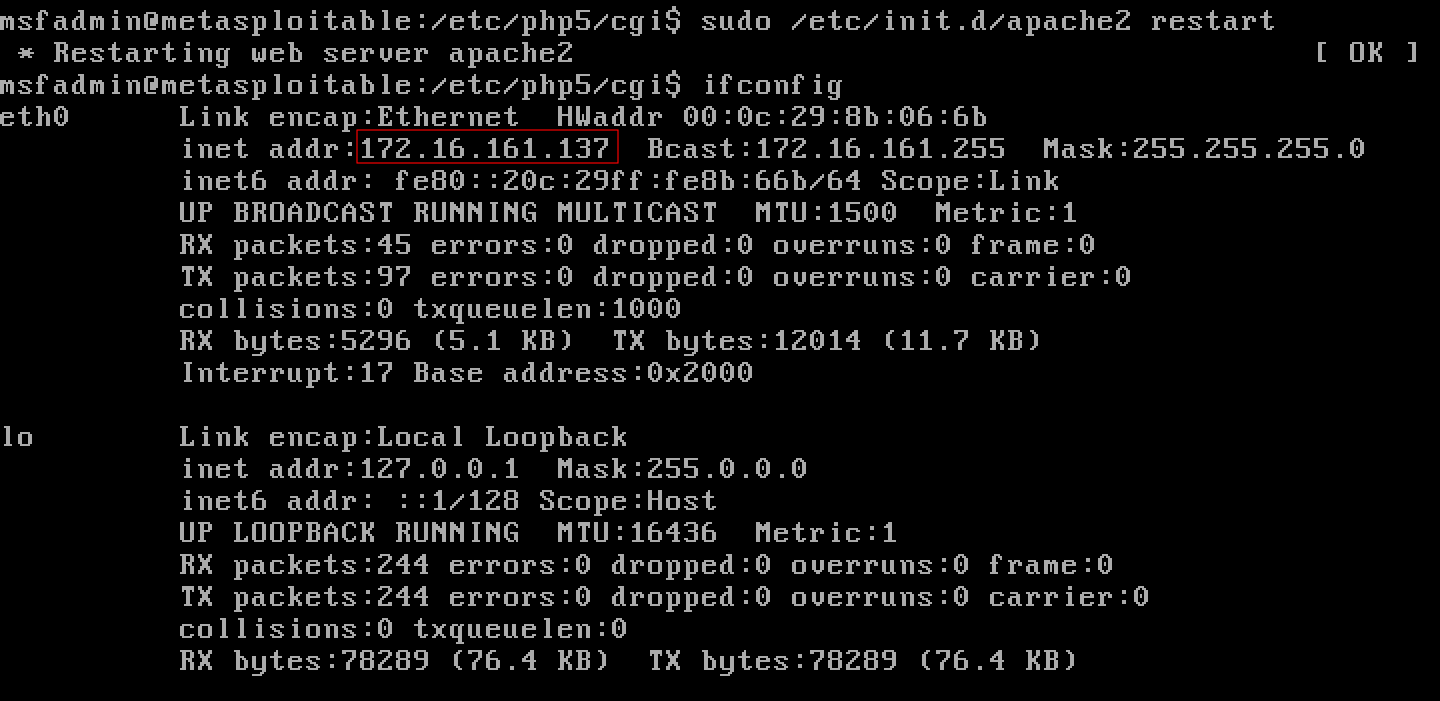
\includegraphics[scale = 0.31]{fig5.png}
 
  \caption{Reiniciação do servidor e obtençao do respetivo IP}

\end{figure}


Por fim podemos aceder ao site usando o URL \textit{"http://172.16.161.137/mutillidae/"} no Firefox.

\begin{figure}[H]

  \centering

  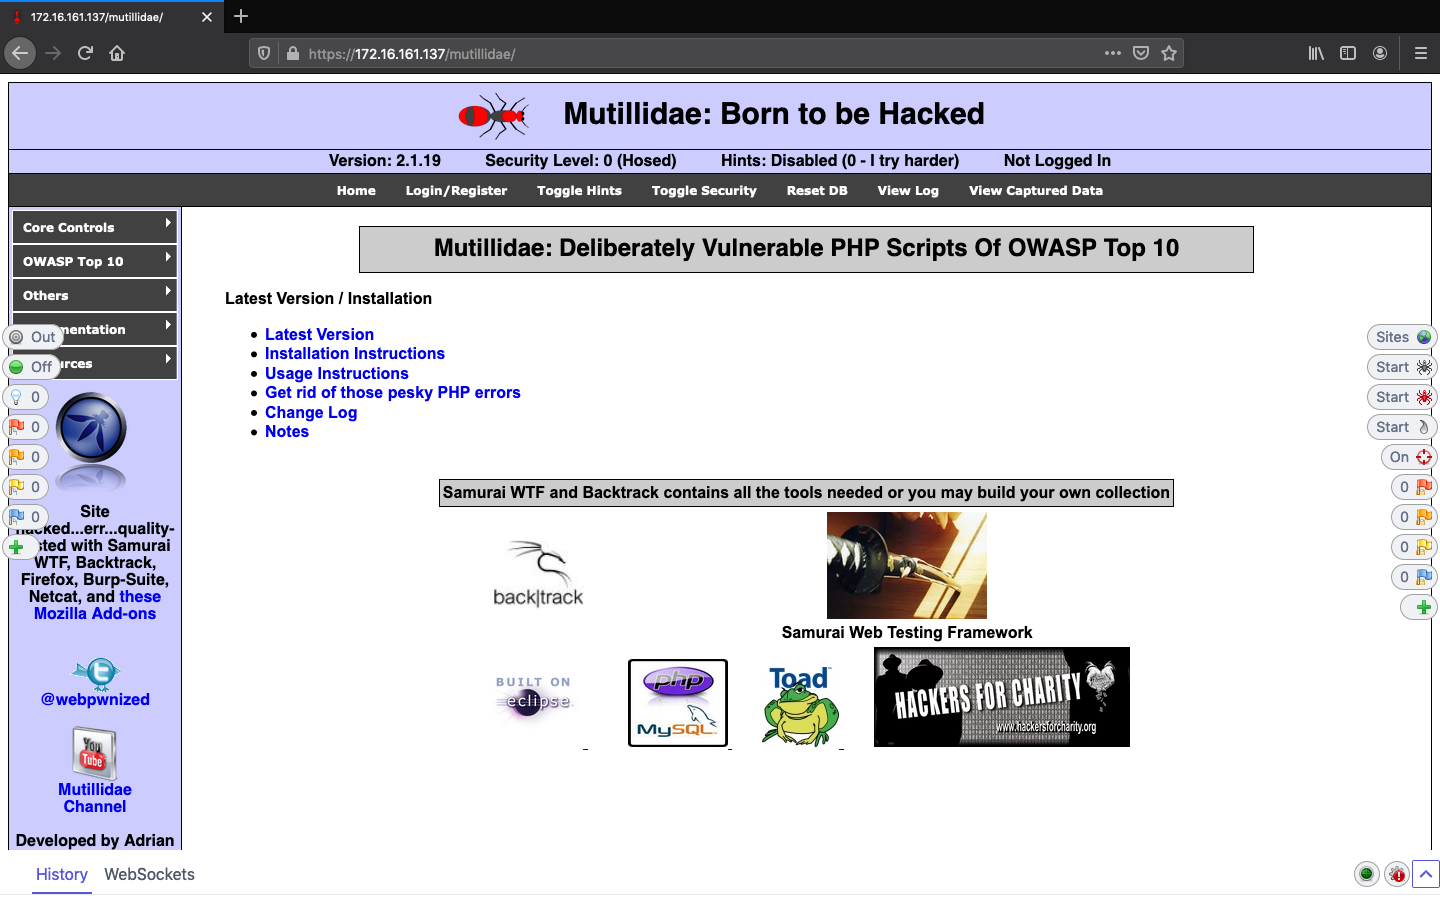
\includegraphics[scale = 0.31]{fig6.png}

  \caption{Acesso ao site multillidae}

\end{figure}

\subsubsection{Firefox}

Agora temos de configurar o Firefox para permitir que o ZAP apanhe as trocas de pedidos e respostas entre o Firefox e o Servidor.
Primerio temos de ir ás definições de rede do browser e configurar as definições de ligação.
\begin{figure}[H]

  \centering

  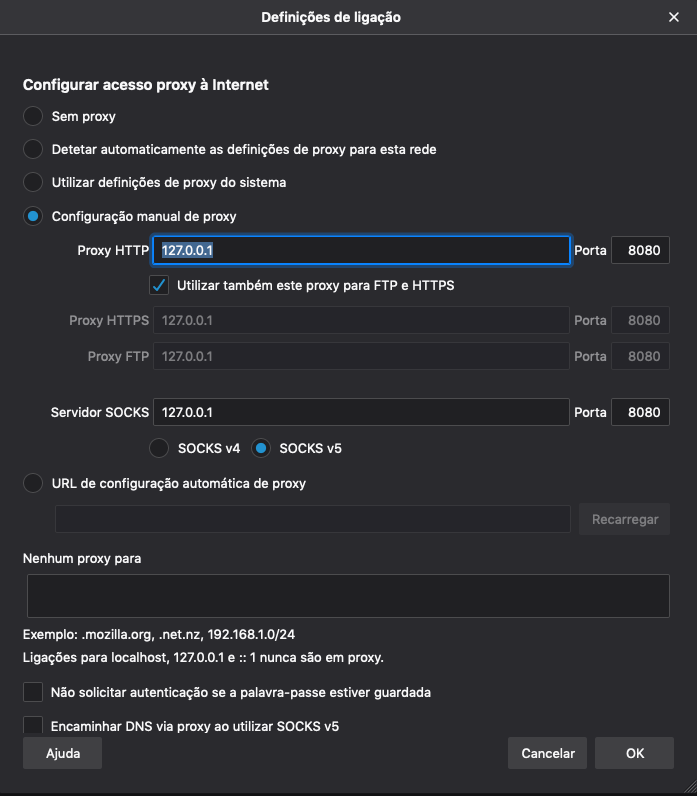
\includegraphics[scale = 0.31]{fig7.png}

  \caption{Definições de ligação do Firefox}

\end{figure}

Como vamos usar o OWASP ZAP temos de importar um certificado do mesmo. Podemos gerar um certificado e guarda-lo onde queremos para adicionar á lista de certificados de confiança do Firefox.

\begin{figure}[H]

  \centering

  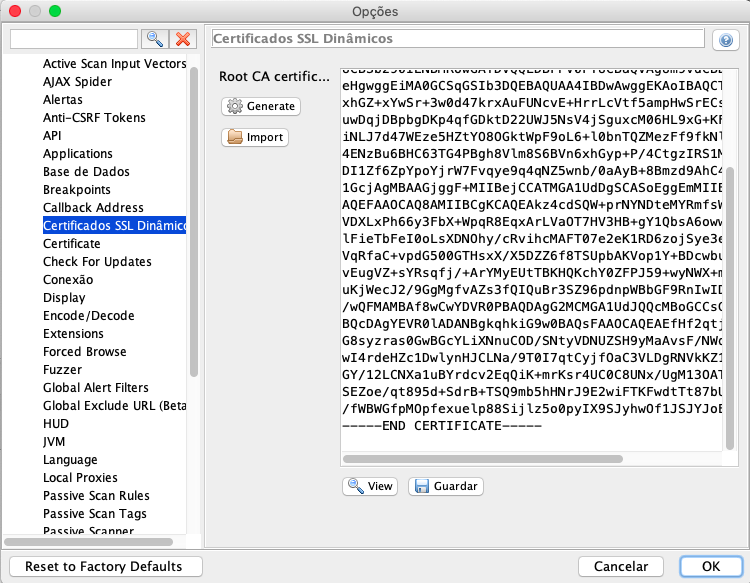
\includegraphics[scale = 0.31]{fig8.png}

  \caption{Geração do certificado SSL}

\end{figure}

Como referido anteriormente, agora basta-nos adicionar o certificado á lista de certificados confiaveis do firefox e podemos aceder ao site que preparamos através do mesmo sendo a informação recolhida pelo OWASP ZAP.

\begin{figure}[H]

  \centering

  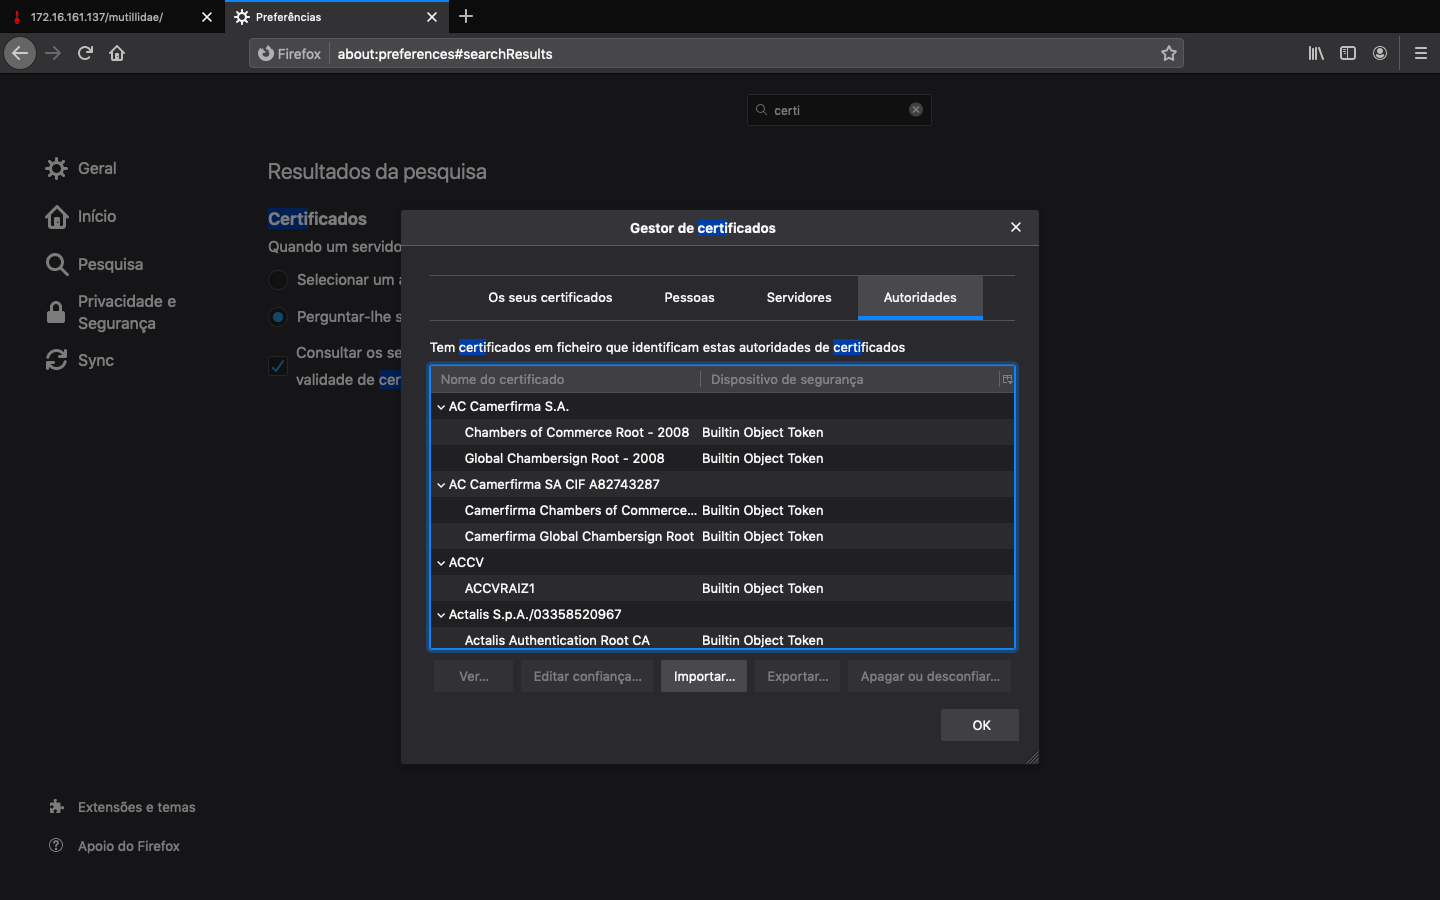
\includegraphics[scale = 0.31]{fig9.png}

  \caption{Adição do certificado SSL aos certificados de confiança do Firefox}

\end{figure}
\begin{figure}[H]

  \centering

  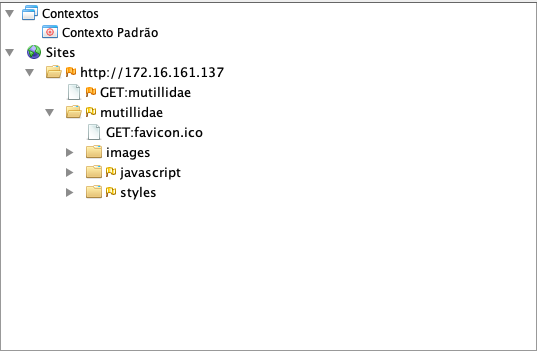
\includegraphics[scale = 0.31]{fig10.png}

  \caption{Informação do acesso ao site através do Firefox coletada pelo ZAP}

\end{figure}



\subsection{Análises}

Nesta secção efetuaremos scans ao servidor apache na máquina virtual metasploitable que corre o mutillidae.\newline

\par Os exemplos de testes que figuram neste relatório, estao divididos em duas categorias, exemplos básicos e exemplos avançados e são:
\begin{itemize}
  \item Exemplos Básicos:
  \begin{itemize}
    \item Spider a website
    \item Fuzz a website
    \item Scan Ativo
    \item Mapear websites autenticados com Ajax
  \end{itemize}

  \item Exemplos Avançados:
  \begin{itemize}
    \item SQL Injections
    \item Brute Force
    \item Cross Site Scripting
    \item Obter ficheiros escondidos no Servidor
  \end{itemize}
\end{itemize}



%################################################################################################


%##################################### BASIC EXEAMPLES ##########################################


%################################################################################################




%######################################### SPIDER ###############################################


\subsubsection{Spider a website}

Spider é um scan passivo e inofencivo destinado a procurar em pedidos e respostas falhas como security headers ou anti CSRF tokens em falta. 
Vamos então realizar esta procura passiva fazendo uso do ZAP.
\begin{figure}[H]

  \centering

  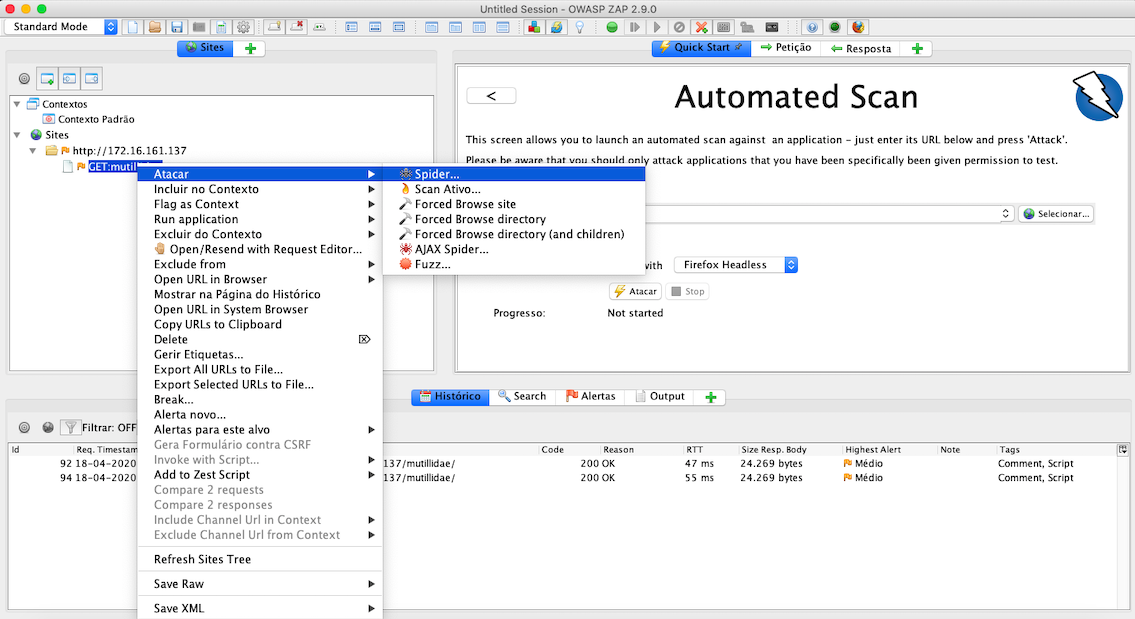
\includegraphics[scale = 0.31]{fig11.png}

  \caption{Procedimento para realizar um Spider Scan}

\end{figure}

Após termos realizado este procedimento podemos ver uma alteração na janela que mostrava os sites vistos.
\begin{figure}[H]

  \centering

  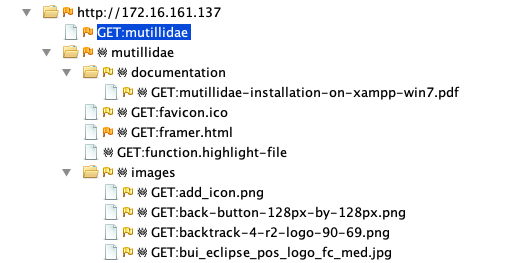
\includegraphics[scale = 0.31]{fig12_1.png}
  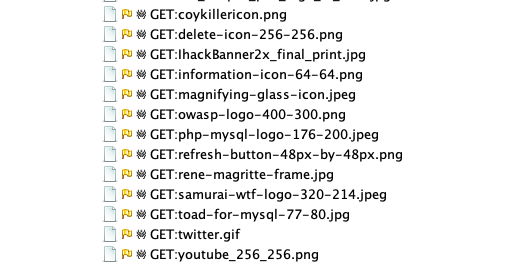
\includegraphics[scale = 0.31]{fig12_2.png}
  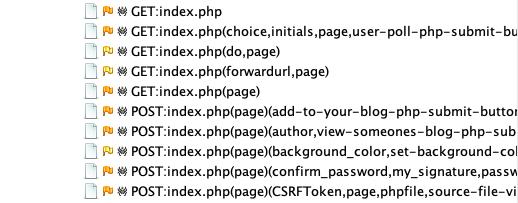
\includegraphics[scale = 0.31]{fig12_3.png}

  \caption{Resultado do Spider Scan}

\end{figure}


A cor da bandeira ao lado dos pedidos indica falhas na resposta recebida, quanto mais escura a cor mas grave é a falha.
Também há uma janela onde são reportados os alertas para melhor visualização dos problemas. Em baixo podemos ver o conteúdo dessa janela.
\begin{figure}[H]

  \centering

  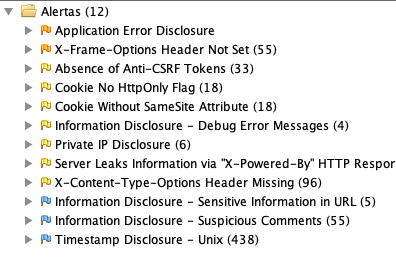
\includegraphics[scale = 0.31]{fig12_4.png}

  \caption{Alertas resultantes do Scan}

\end{figure}

%######################################### Fuzzering ##############################################


\subsubsection{Fuzz a website}


Para fins demonstrativos vamos usar a página de login para realizar o ataque fuzz. Nas figuras segunites vemos o resultado de tentar fazer login no servidor mutillidae com o username \textit{admin} e a password \textit{wrongPassword} bem como o respetivo pedido apanhado pelo ZAP.
\begin{figure}[H]

  \centering

  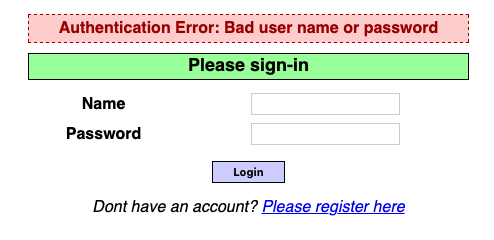
\includegraphics[scale = 0.31]{fig22.png}

  \caption{Formulario de autenticação}

\end{figure}
\begin{figure}[H]

  \centering

  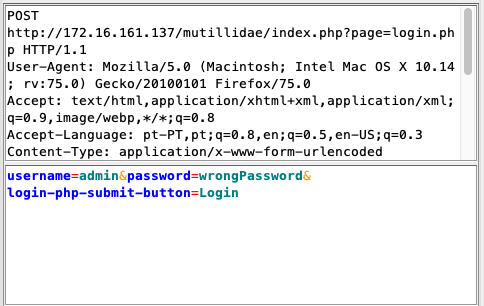
\includegraphics[scale = 0.31]{fig23.png}

  \caption{Pedido de autenticação submetido}

\end{figure}

Agora para realizarmos o fuzz temos de selecionar o pedido apanhado pelo ZAP com o username e a password errados e fazendo uso das opções disponibilizadas pelo botão direito do rato escolher Fuzz.

\begin{figure}[H]

  \centering

  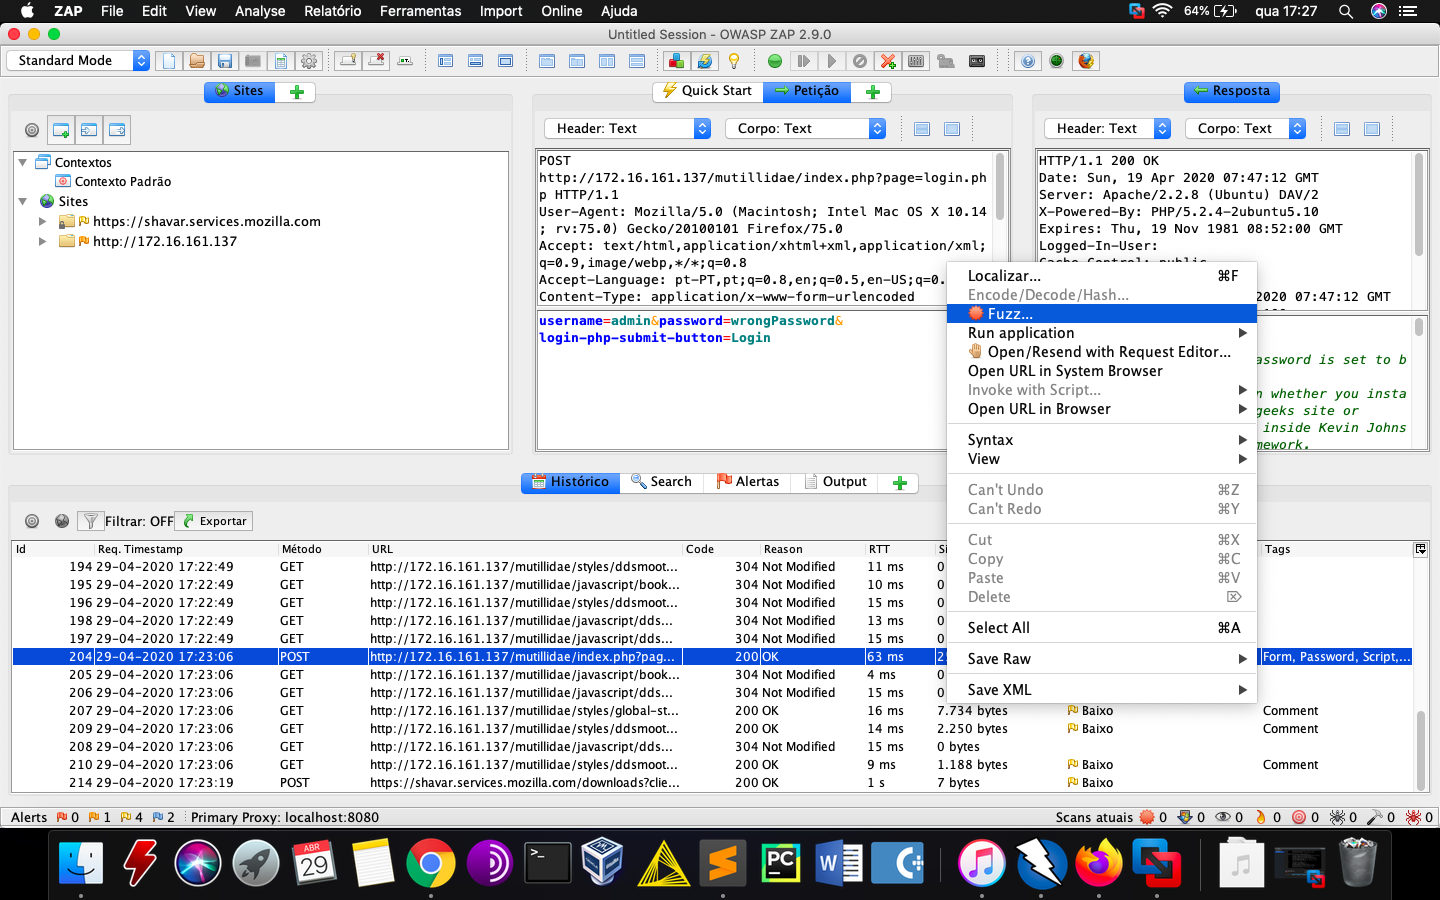
\includegraphics[scale = 0.31]{fig24.png}

  \caption{Abertura da janela de configuração do Fuzzer}

\end{figure}

Agora com a janela do fuzz aberta basta-nos selecionar o campo sobre o qual queremos executar o fuzz na mensage interceptada e carregar um payload para substituição. Neste caso como estamos a falar de um autenticaçao vamos escolher a opção \textit{File Fuzzers} e dentro desta escolher \textit{injeção SQL} e dentro de todas as opções vamos escolher apenas duas para manter o teste simples. Note-se que na segunda figura podemos ver no campo \textit{Payloads Preview} onde é mostrado o que será registado no campo.

\begin{figure}[H]

  \centering

  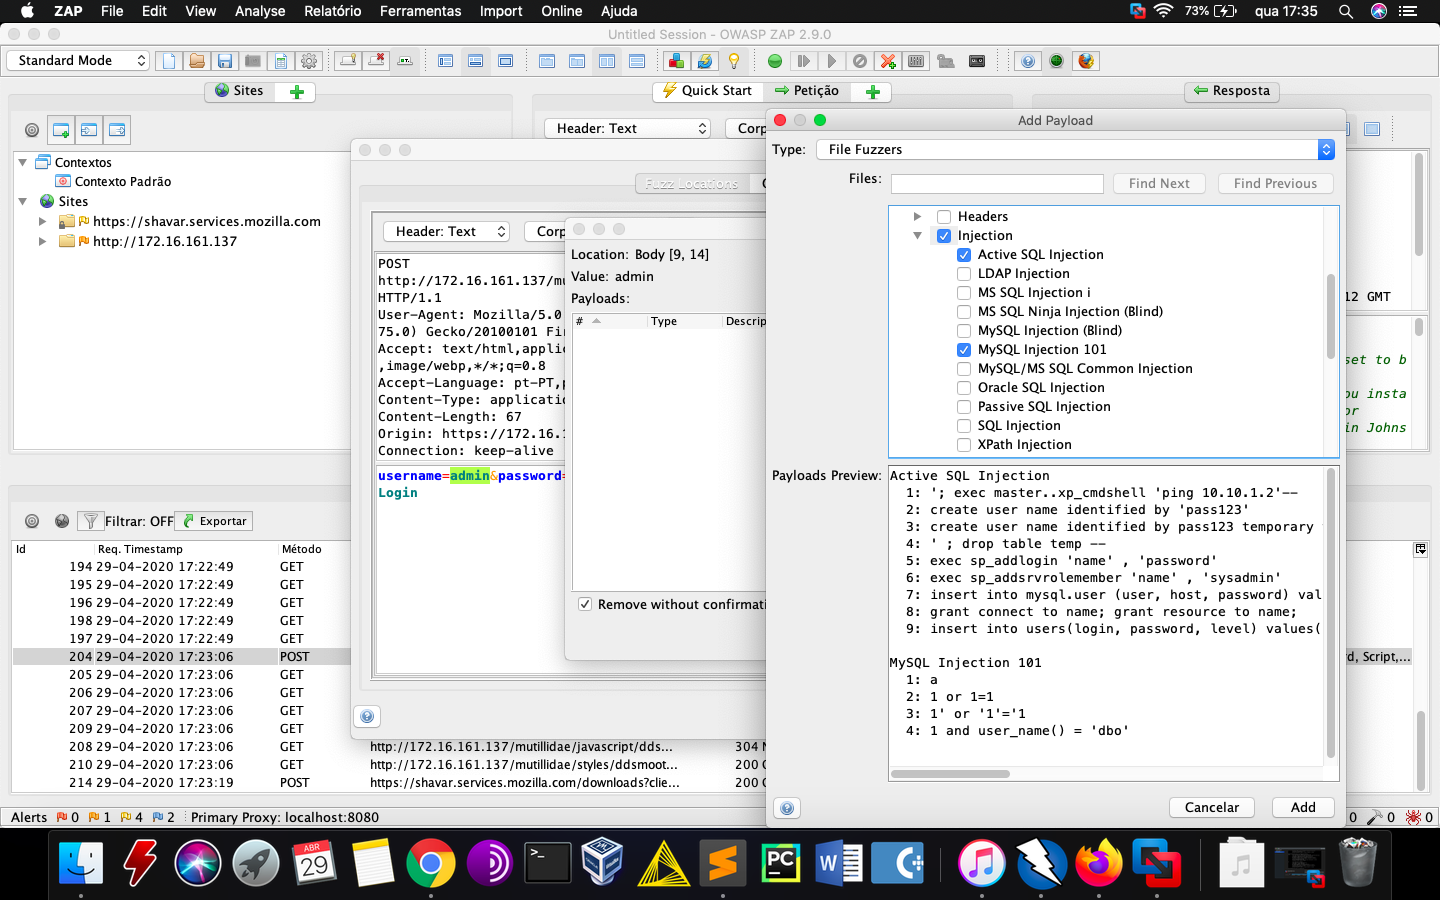
\includegraphics[scale = 0.31]{fig26.png}

  \caption{Configuração escolhida para o Fuzzer}

\end{figure}

Após escolhermos as opções basta carregar no botão \textit{Start Fuzzer} e esperar. Como o fuzzer executa rápido obtemos respostas que podem ser ordenadas pelo tamanho de corpo de resposta e nas quais podemos ver o payload. Para uma busca mais eficaz podemos usar a barra search sobre o tipo \textit{HTTP Fuzzer Results} para procurar palavras especificas como \textit{error} ou \textit{syntax}. Neste caso usamos a palavra syntax e se repararmos temos o campo username substituido por uma pelica, o que causa um erro no servidor. Se fizermos a substituição e submetermos o formulário de login na página acabamos por confirmar a existencia de um erro como se vê nas figuras abaixo.

\begin{figure}[H]

  \centering

  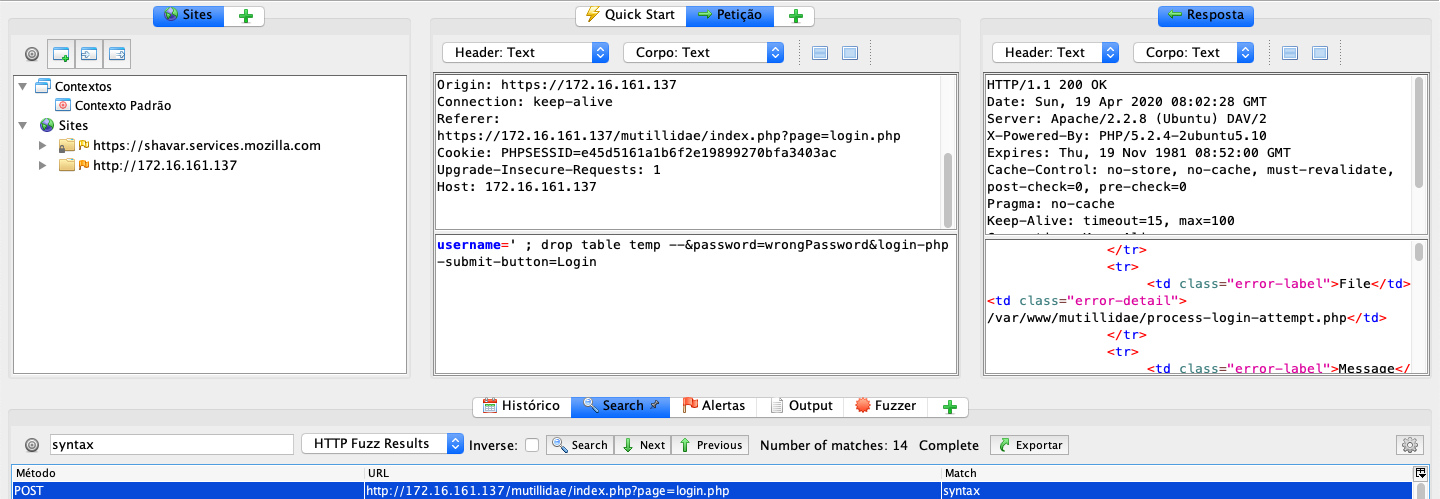
\includegraphics[scale = 0.31]{fig28.png}

  \caption{Exemplo de substituição do username}

\end{figure}
\begin{figure}[H]

  \centering

  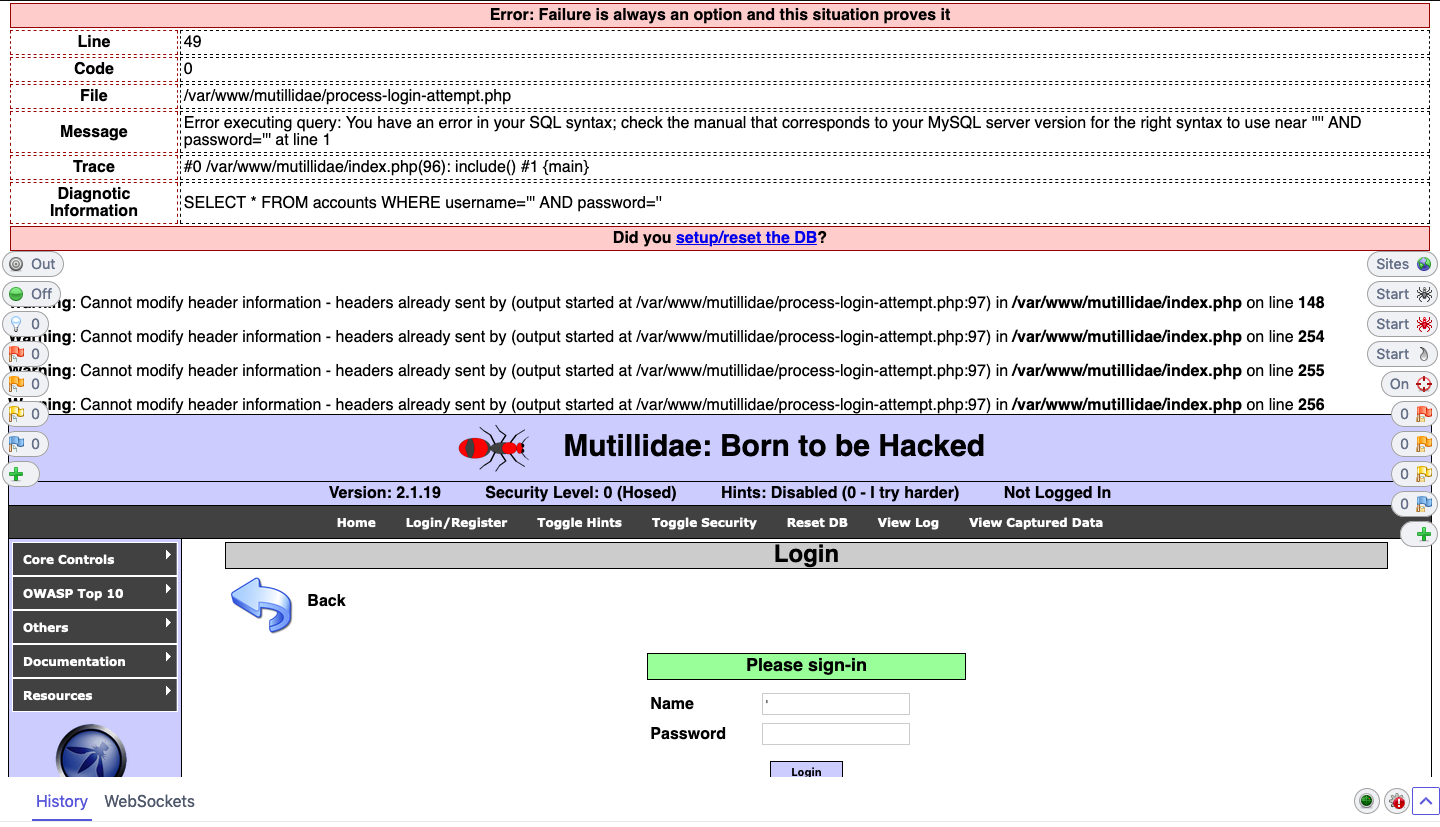
\includegraphics[scale = 0.31]{fig29.png}

  \caption{Resultado da substituição do username}

\end{figure}

Para além disso note-se também que obtivemos informação útil sobre a base de dados. Agora sabemos que existe uma tabela SQL chamada accounts com os campos username e password.



\subsubsection{Scan ativo}

Para fazer o scan ativo basta-nos simplesmente escolher um site e selecionar a opção scan ativo, este correrá um scan padrão pré-definido no ZAP.

\begin{figure}[H]

  \centering

  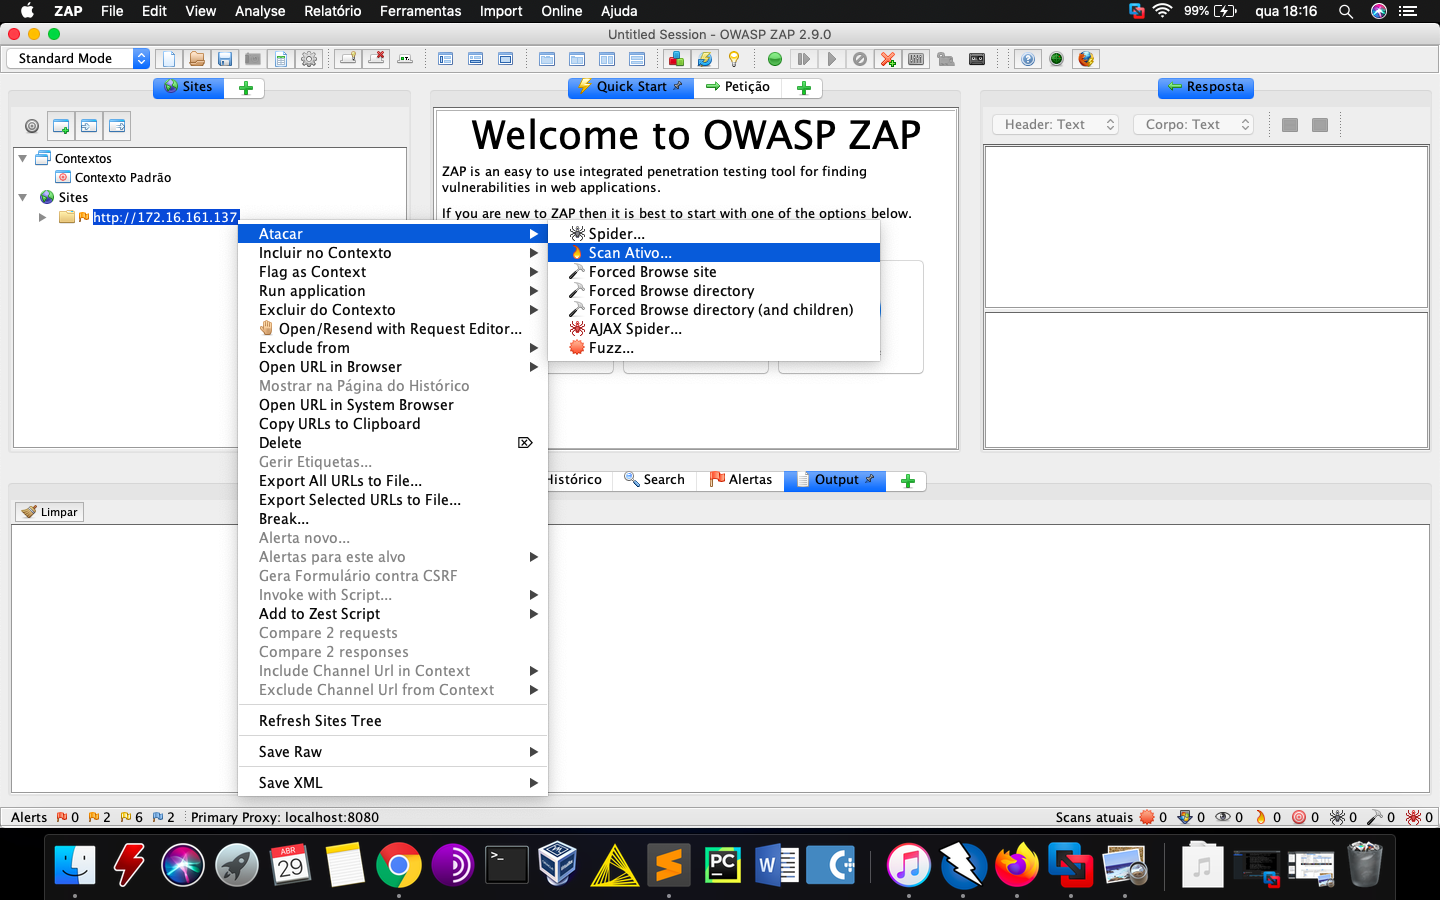
\includegraphics[scale = 0.31]{fig34.png}

  \caption{Procedimento para realizar um Scan Ativo}

\end{figure}


 Podemos ver o resultado do mesmo na figura abaixo, onde na tab Alertas obtemos todos os alertas que o scan padrão detetou etiquetadas pela gravidade da falha identificada pela cor da bandeira.

\begin{figure}[H]

  \centering

  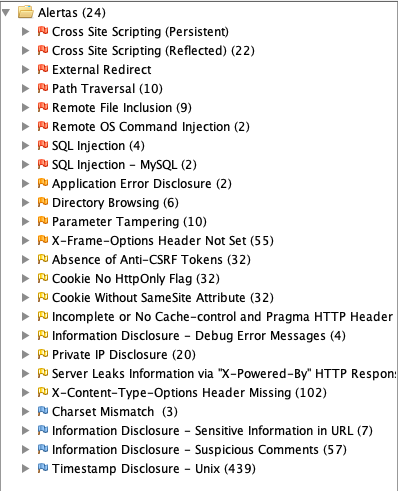
\includegraphics[scale = 0.31]{fig17.png}

  \caption{Alertas resultantes de realizar um Scan ativo}

\end{figure}


%###################################### AJAX ############################################


\subsubsection{Mapeamento de websites com autenticação de utilizador usando Ajax}

A vantegem desta técnica de Spider é podermos aceder a URLs aos quais apenas utilizadores autenticados podem aceder, originando assim um mapeamento mais detalhado da organização do site.\newline
O primeiro passo para realizar este teste é ter descoberto uma combinação username-password válida e realizar a autenticação. Caso ainda não tenha realizado este passo por favor veja a subsecção de Brute Force.\newline
Para garantir que se está auntenticado caso observemos a tab HTTP session devemos ver uma imagem parecida com a seguinte.\newline

\begin{figure}[H]

  \centering

  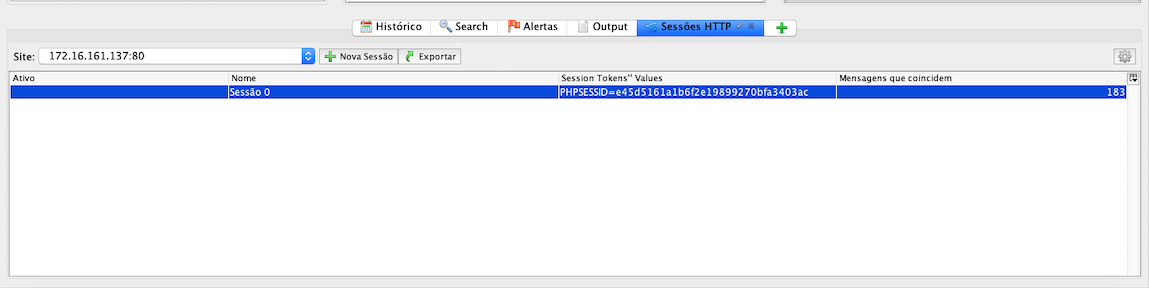
\includegraphics[scale = 0.31]{fig35.png}

  \caption{Sessão HTTP por ativar}

\end{figure}

Devemos então clicar na barra correspondente á seção atual na janela e definir a mesma como ativa. Posteriormente na janela onde visualizamos os sites visitados devemos selecionar aquele com a sessão ativa e escolher a opção \textit{Ajax Spider}. Desta forma o Ajax usará a nossa conta para realizar o Spider do website. Para além disso o Ajax Spider reautentica-se para garantir que caso exista a opção de \textit{log off} o utilizador não seja desconectado.

\begin{figure}[H]

  \centering

  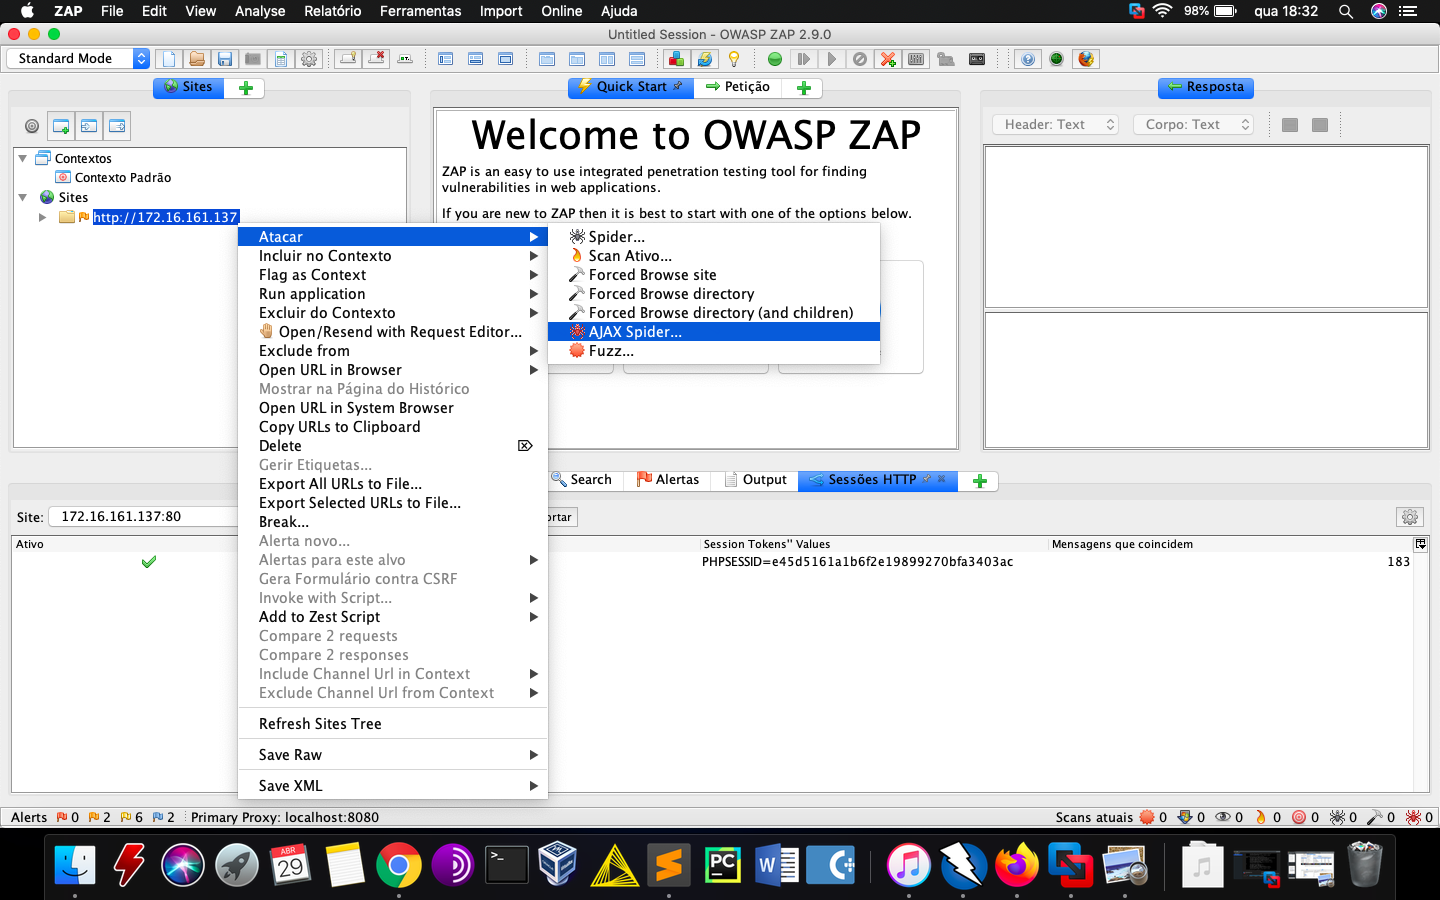
\includegraphics[scale = 0.31]{fig36.png}

  \caption{Procedimento para realizar um mapeamento com Ajax após ativação da sessão}

\end{figure}

Por fim podemos ver os pedidos realizados pelo \textit{Ajax} na janela inferior do ZAP bem como aceder á configuração do site alvo na tab correspondente aos sites.  

\begin{figure}[H]

  \centering

  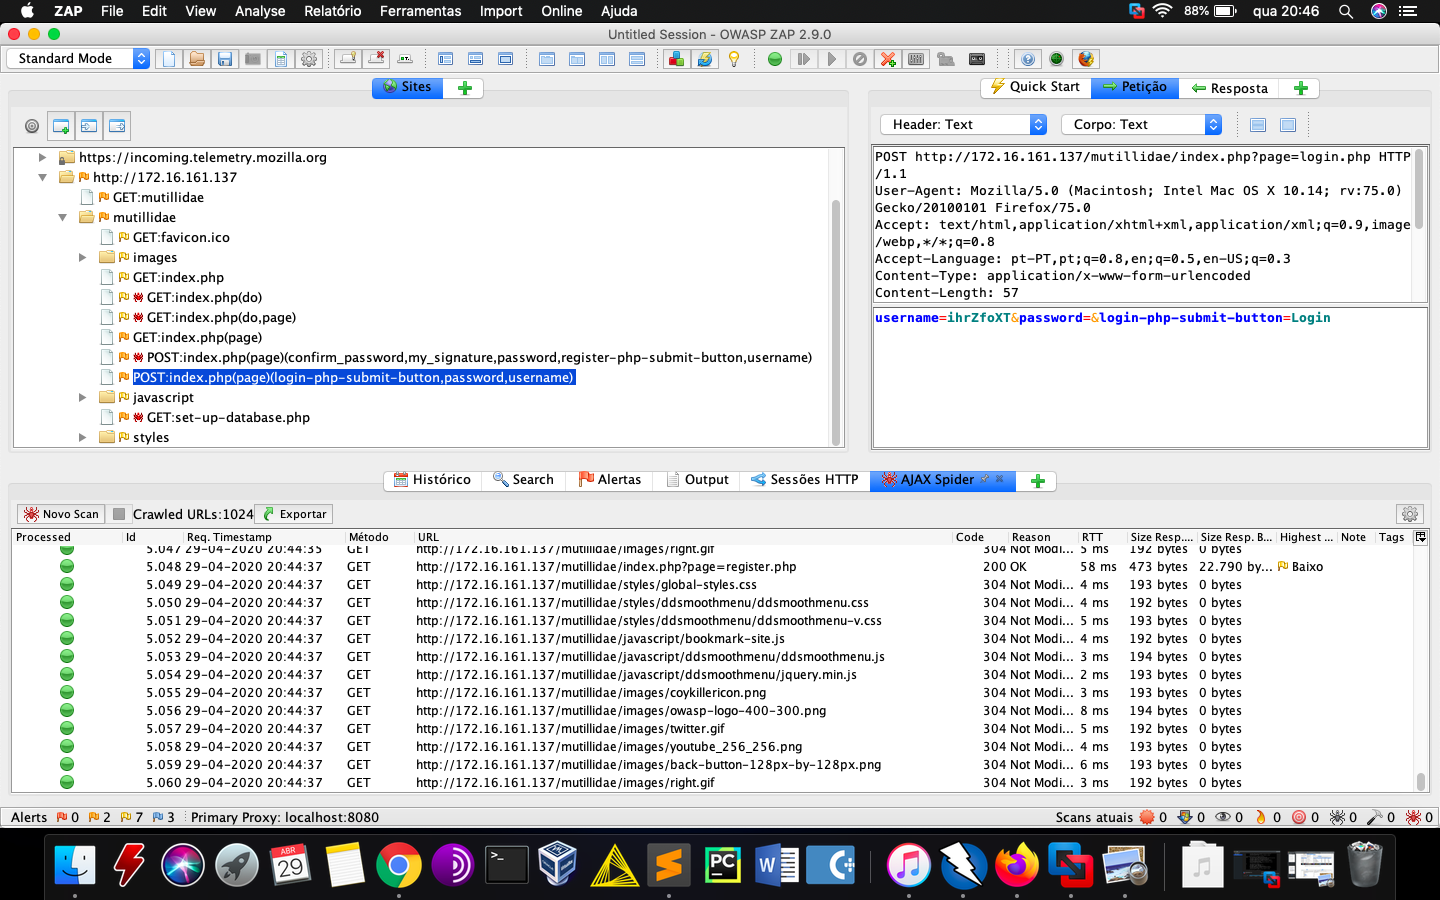
\includegraphics[scale = 0.31]{fig37.png}

  \caption{Site mapeado e pedidos feitos pelo Ajax}

\end{figure}




%################################################################################################


%################################### ADVANCED EXEAMPLES #########################################


%################################################################################################


\subsubsection{SQL Injections}

O propósito deste exemplo e demonstrar como injeções de código SQL podem comprometer a segurança. Primeiro vamos autenticar-nos no site e executar um scan ativo para testar o mesmo, como o ZAP esteve a guardar tudo em background ao executar o scan pode revelar mensagens interessantes. Como se pode ver na imagem temos 2 alertas de possiveis injeções de código SQL.




\begin{figure}[H]

  \centering

  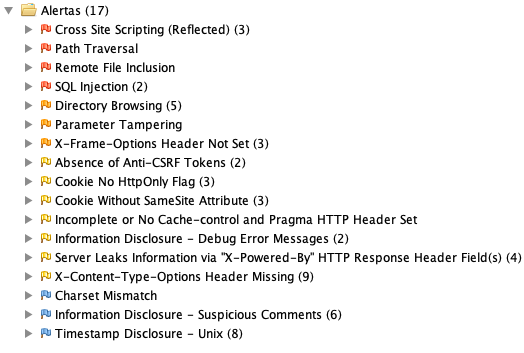
\includegraphics[scale = 0.31]{fig39.png}

  \caption{Alertas resultantes do Scan Ativo}

\end{figure}

Se nos aprofundarmos nos alertas podemos inspecionar o alerta e obter mais informação sobre a falha.


\begin{figure}[H]

  \centering

  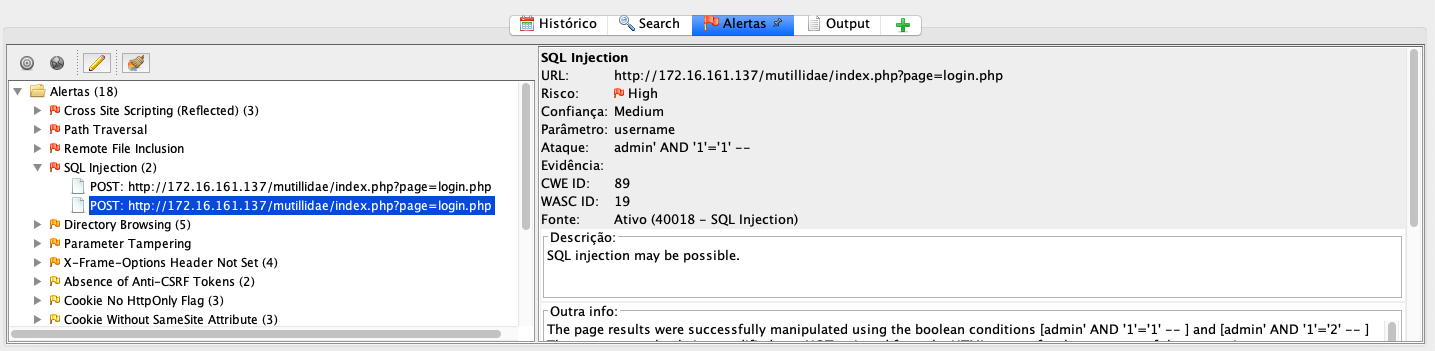
\includegraphics[scale = 0.31]{fig40.png}

  \caption{Alertas de SQL injection}

\end{figure}


Agora, basta-nos selecionar o campo do username e selecionar Fuzzer. No Fuzzer basta-nos adicionar uma nova \textit{Fuzzer Location} carregando no botão add na janela do \textit{Fuzzer}. Em seguida escolhemos todos os tipos de injeções MySQL, começando em seguida o scan. 


\begin{figure}[H]

  \centering

  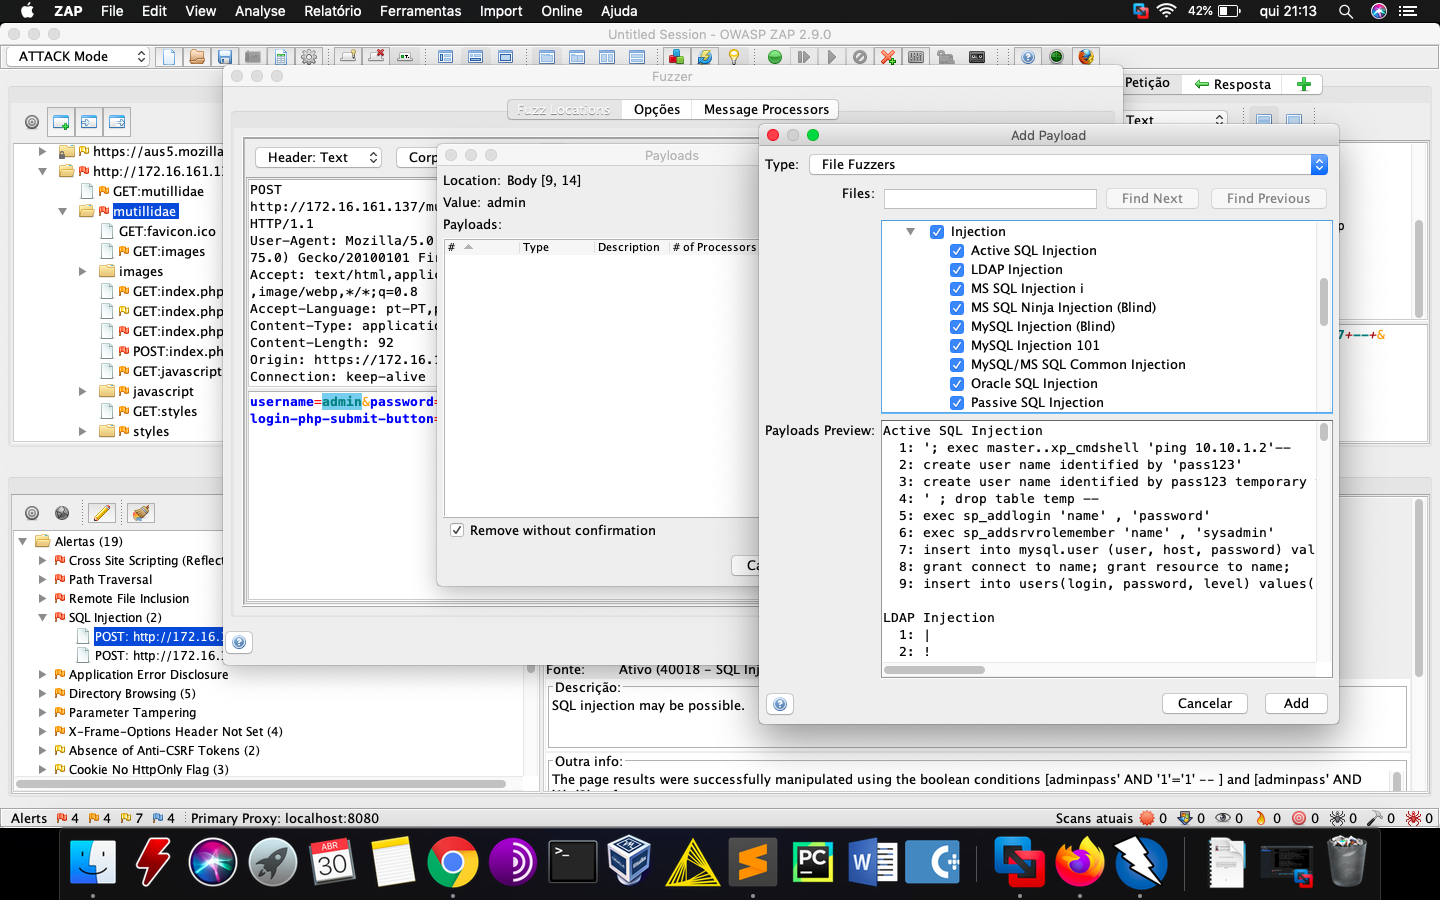
\includegraphics[scale = 0.31]{fig41.png}

  \caption{Configuração do Fuzzer para Injeção de código SQL}

\end{figure}



Se olharmos para uma das mensagens etiquetada com a tag \textit{"Found"}, podemos ver o que o ZAP enviou no formulário. No caso da mensagem que podemos visualizar em baixo foi inserido no campo admin o código: \textit{' or '1'='1}.

\begin{figure}[H]

  \centering

  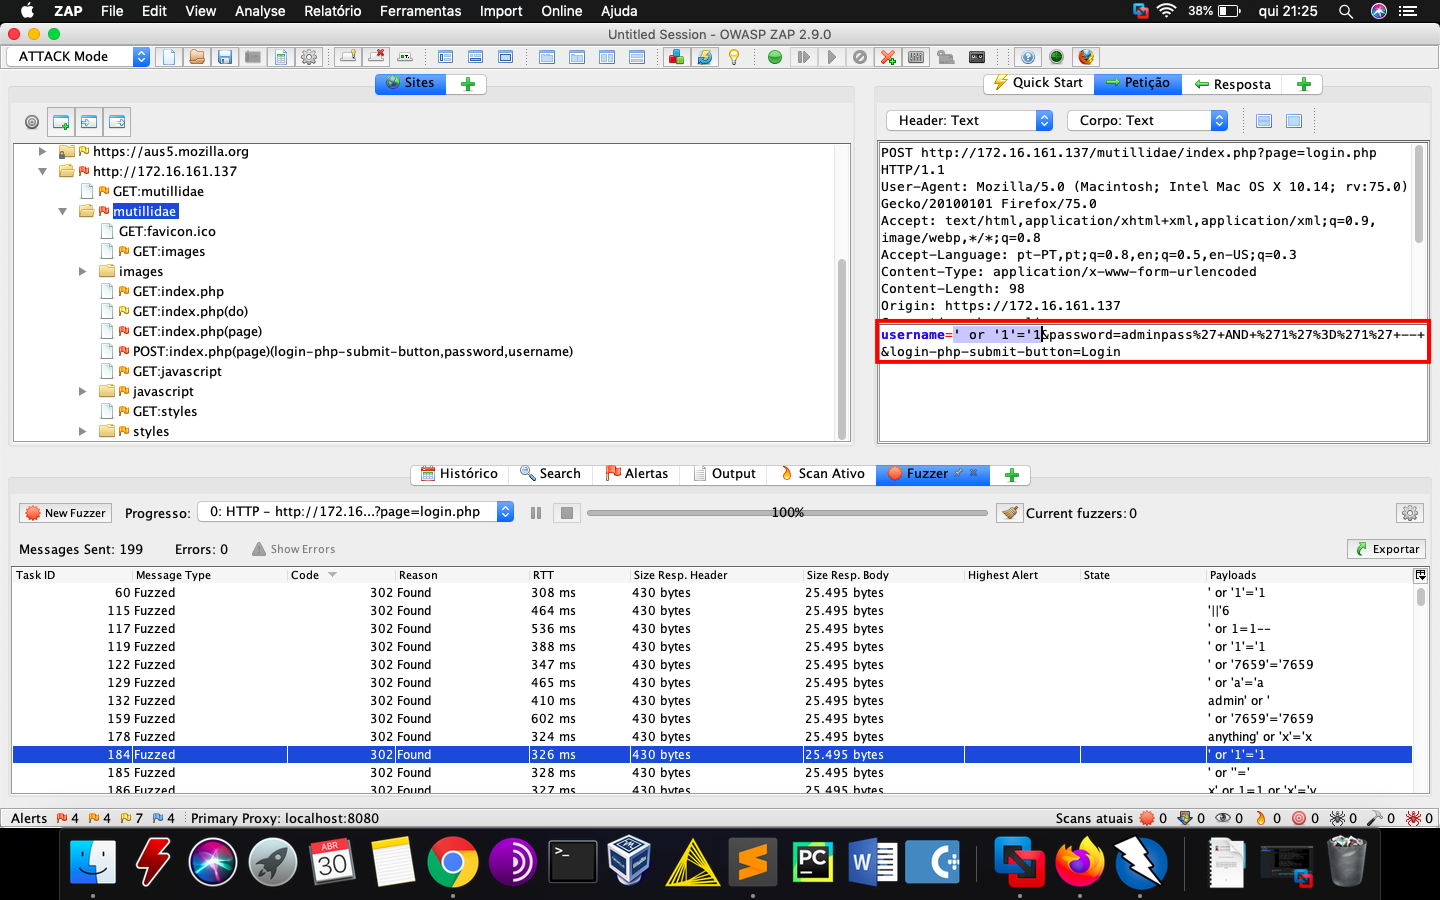
\includegraphics[scale = 0.31]{fig42.png}

  \caption{Exemplo de injeção SQL bem sucedida}

\end{figure}

Se testarmos este código no campo do admin conseguimos acesso ao site.

\begin{figure}[H]

  \centering

  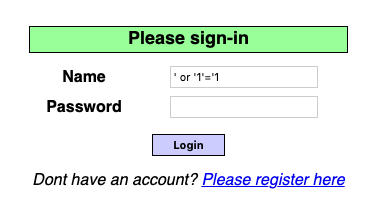
\includegraphics[scale = 0.31]{fig43.png}

  \caption{Injeção de código SQL manual}

\end{figure}
\begin{figure}[H]

  \centering

  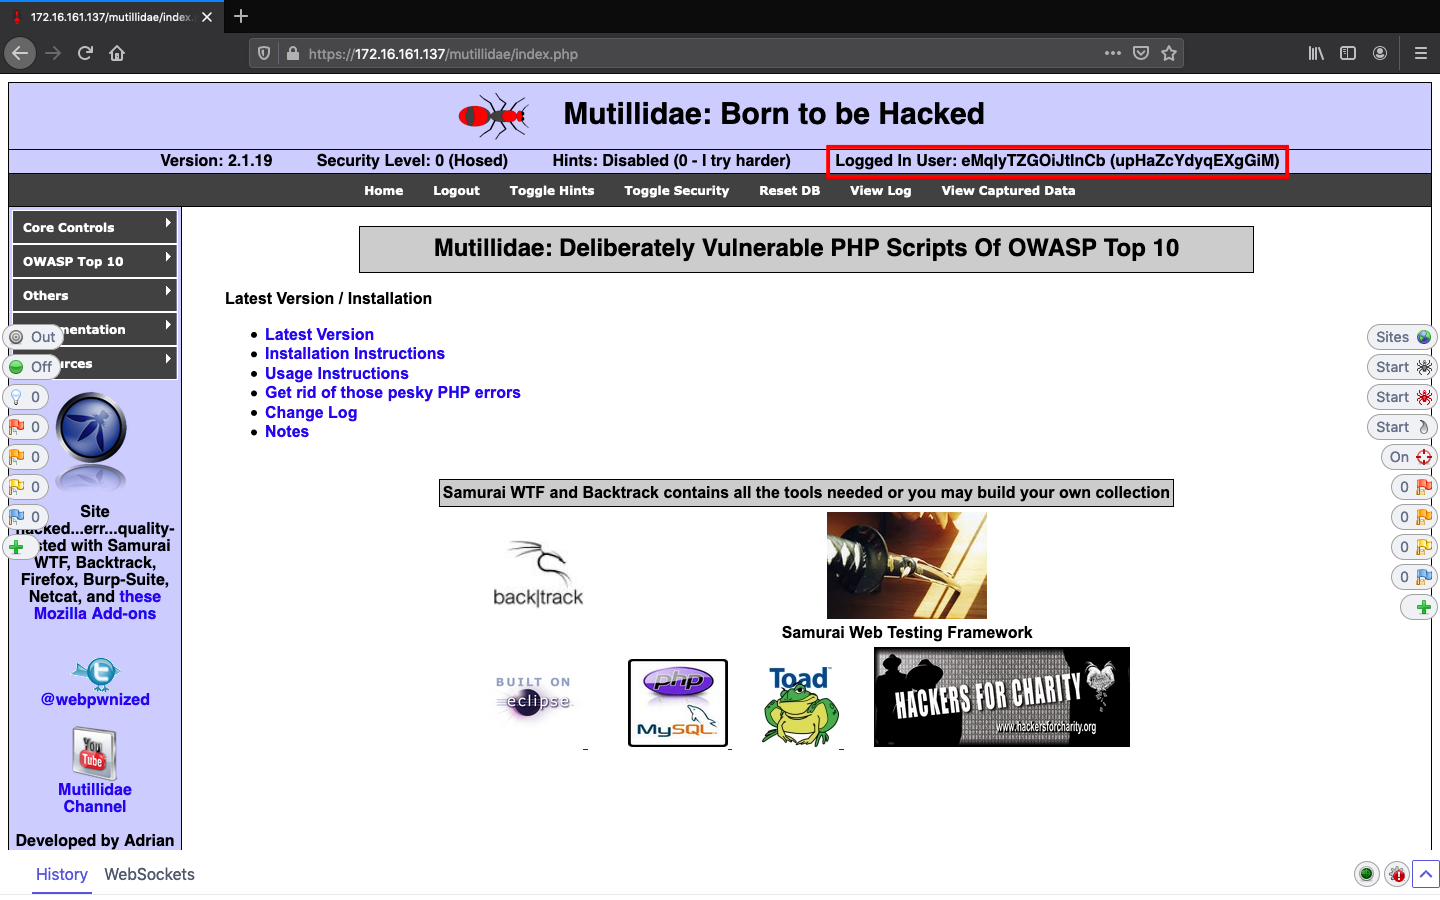
\includegraphics[scale = 0.31]{fig44.png}

  \caption{Login bem sucedido com injeção SQL}

\end{figure}

A lição a tirar neste teste é que não é feita nenhuma verificação do que foi inserido pelo utilizador, ou seja quem desenvolveu o acesso á base de dados confia cegamente no input fornecido pelo utilizador o que permite ataques deste tipo.





\subsection{Ataque Brute Force}

Antes de executarmos este ataque é importante lembrar que este é um teste que demora bastante tempo a executar, por isso convem estar atento a mensagens que aguns sites dão como este \textit{utilizador não existe} ou \textit{password inválida}, que nos dão pistas sobre se devemos respetivamente mudar o username ou tentar passwords diferentes visto que o username existe na base de dados. Por isso devemos começar por tentar obter um username. Digamos que o username que identificamos é : \textit{admin}.
Para executar este ataque á semelhança do exemplo usado com o Fuzzer devemos colocar  no campo de username o username válido e submeter o formulário. Para melhor compreenção o campo password será preenchido com a palavra \textit{"Altera-me"}.
Neste caso tal como no fuzz selecionamos o pedido interceptado e usamos a opção Fuzzer. Na mensagme selecionamos a palavra \textit{Altera-me} e adicionamos um ficheiro pré-gerado com palavras que podem ser uma password correta: \textit{passwords.txt}.


\begin{figure}[H]

  \centering

  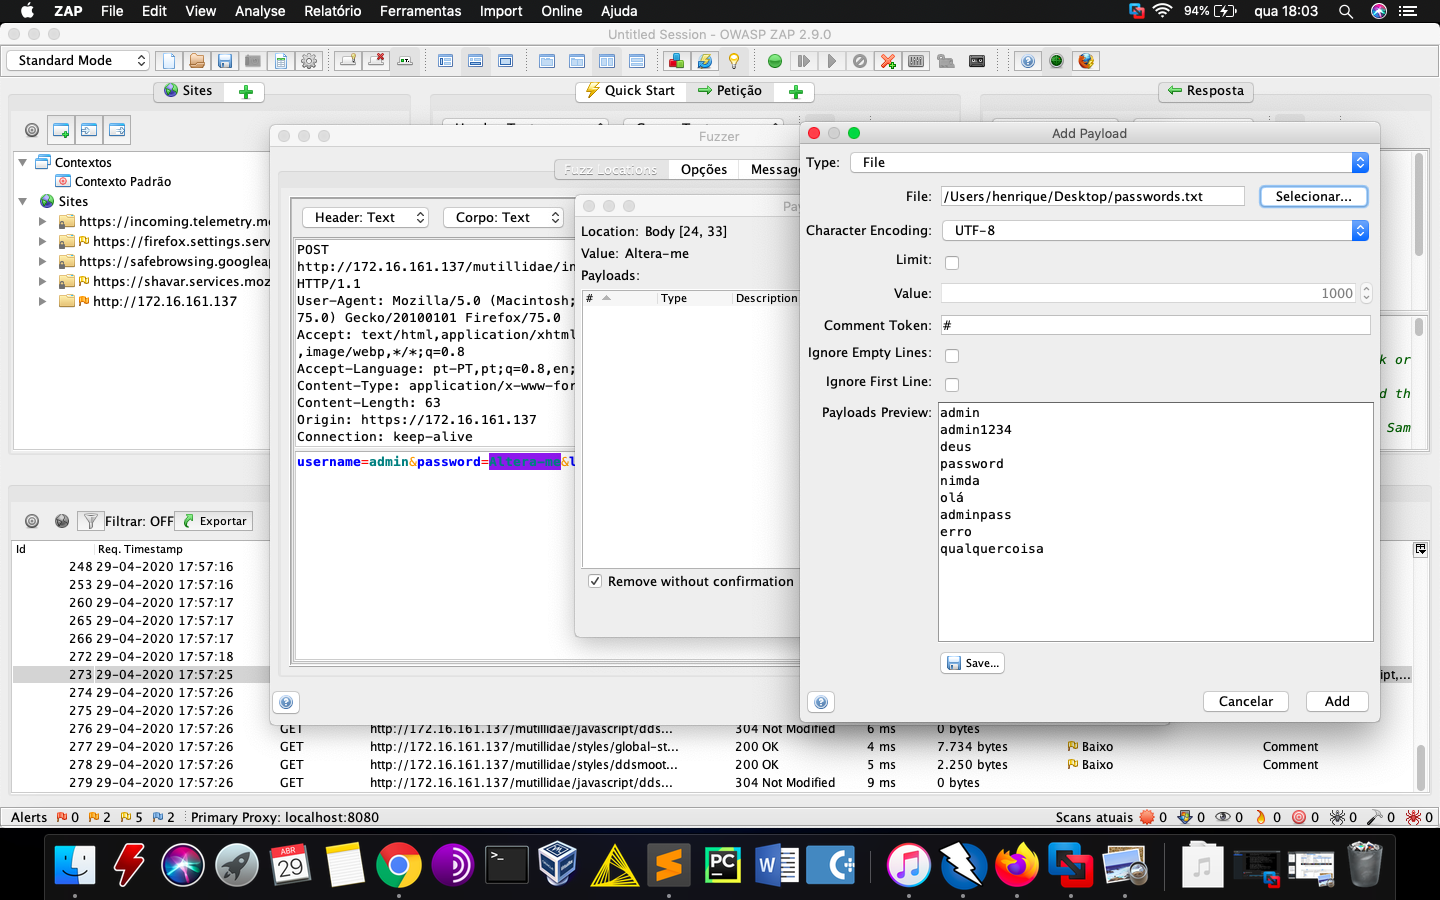
\includegraphics[scale = 0.31]{fig30.png}

  \caption{Configuração do Fuzzer para usar ficheiro pré-gerado de possíveis passwords}

\end{figure}

Para termos uma forma de validação mais simples, caso a password esteja correta, podemos na tab opções escolher "Follow Redirect" para que mal haja uma mudança de página, ou seja, a password inserida foi a correta ou despoletou uma ação que nos levou a uma página diferente, o ZAP pare o scan e possamos observar como o último pacote enviado foi preenchido. Assim podemos tentar substituir a password no site e verificar se é a password correta ou não.

\begin{figure}[H]

  \centering

  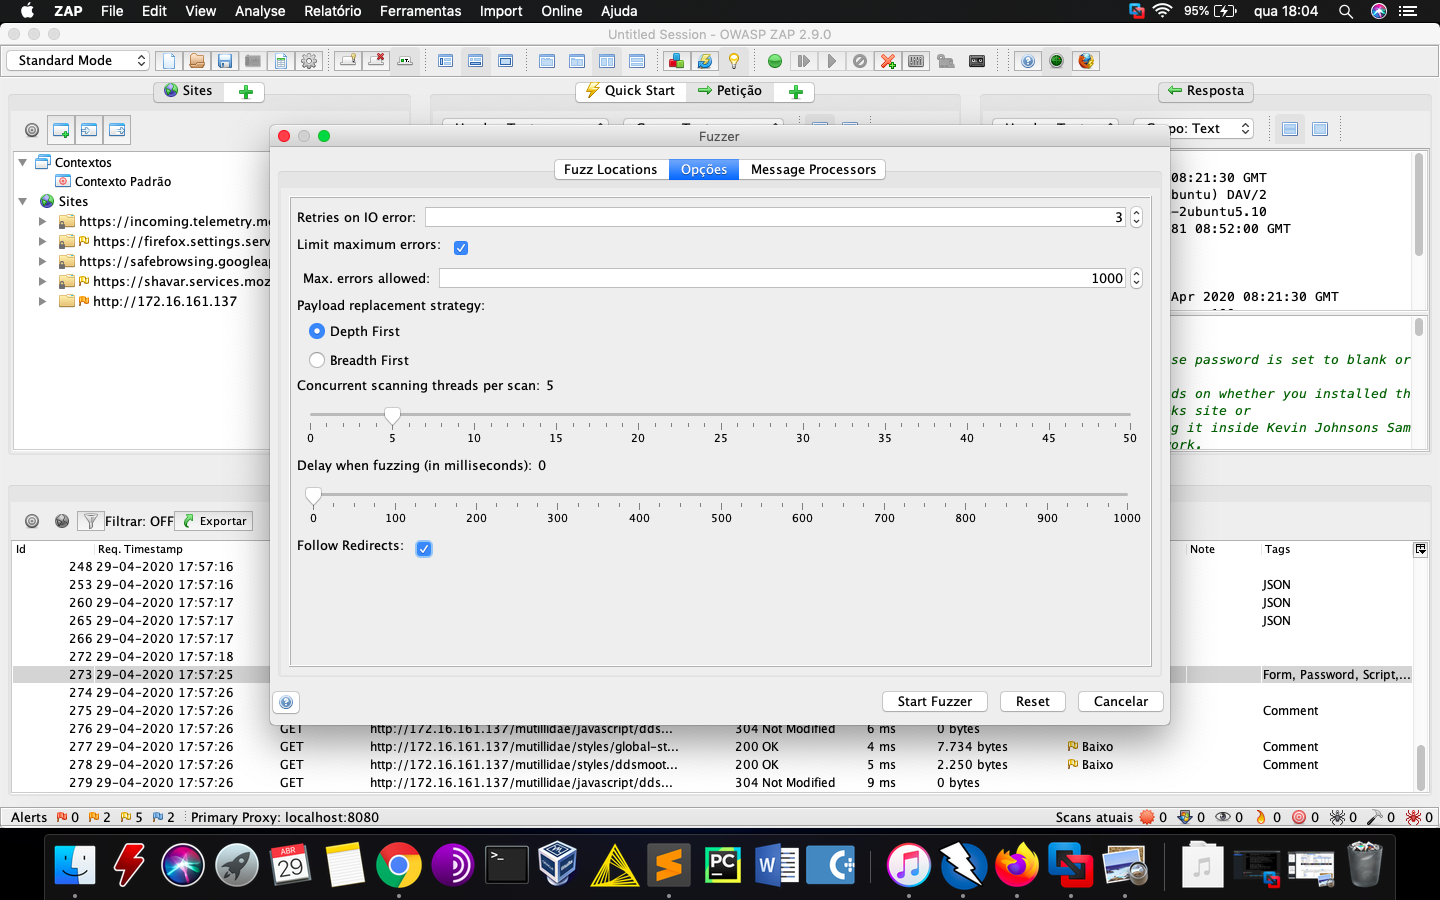
\includegraphics[scale = 0.31]{fig31.png}

  \caption{Configuração para parar no primeiro redirecionamento}

\end{figure}
\begin{figure}[H]

  \centering

  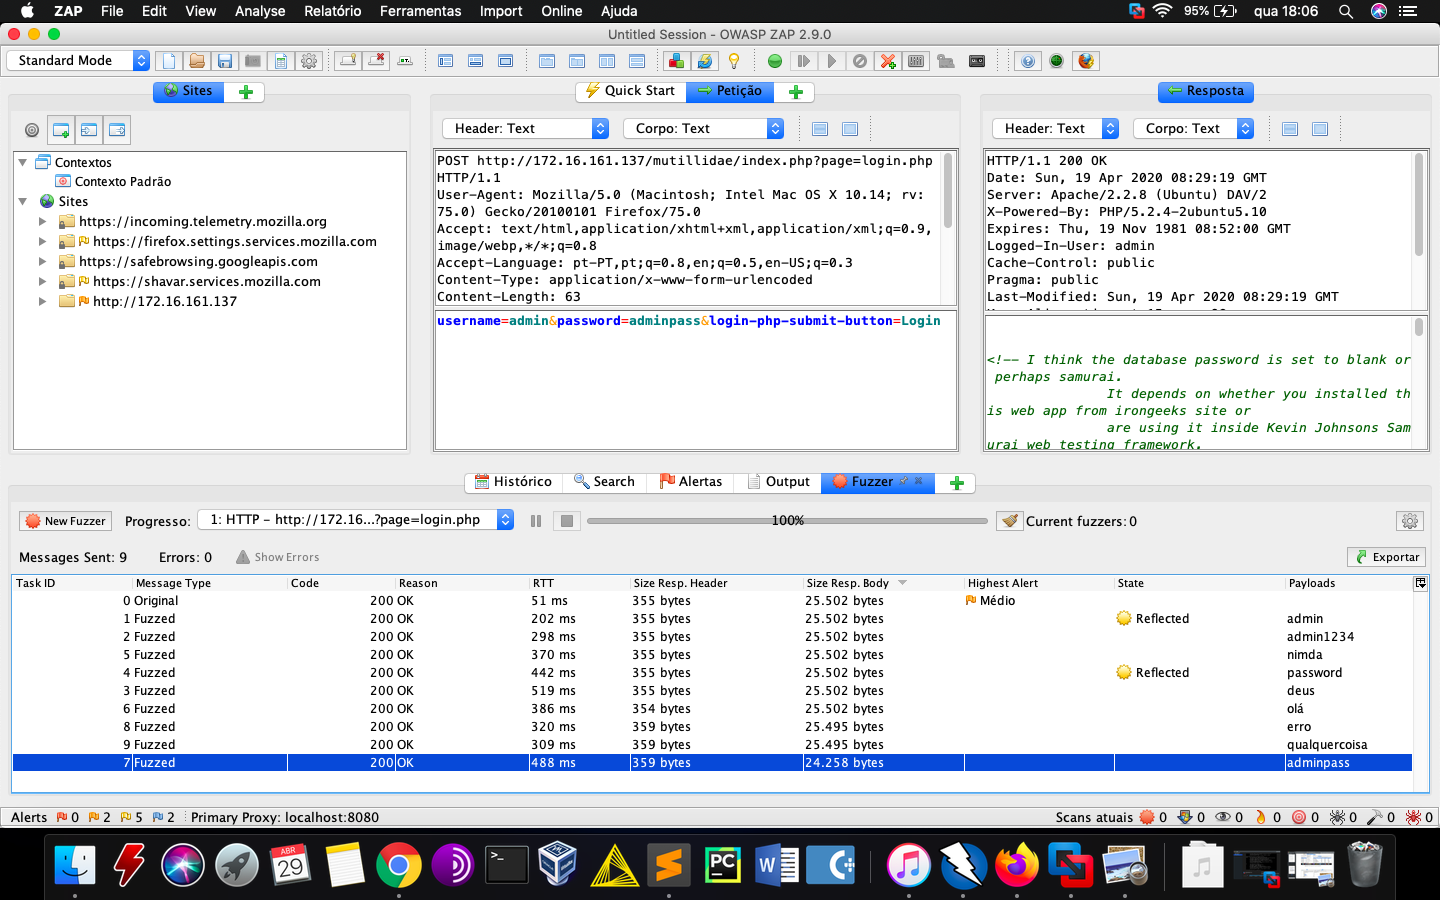
\includegraphics[scale = 0.31]{fig32.png}

  \caption{Resultado em que a página foi redirecionada}

\end{figure}
 Na imagem acima podemos ver que o payload do campo password foi preenchido com a palavra \textit{adminpass}, assim ao testarmos na página confirmamos que de facto esta é a password correta.

\begin{figure}[H]

  \centering

  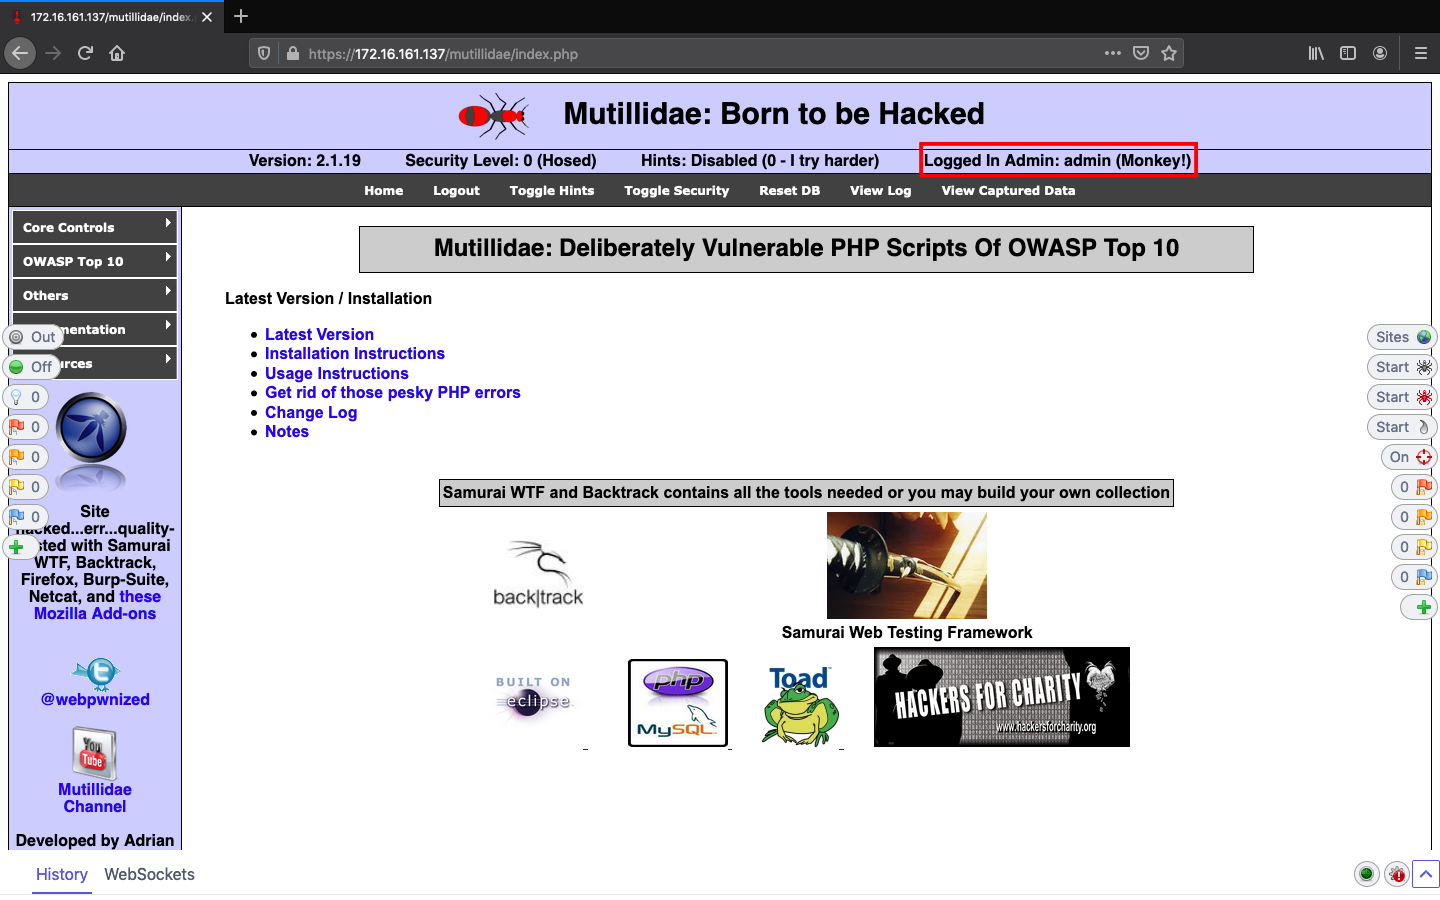
\includegraphics[scale = 0.31]{fig33.png}

  \caption{Resultadod do teste do resultado anterior no site}

\end{figure}


%################################## CROSS SITE SCRIPTING ########################################


\subsubsection{Cross Site Scripting}

Neste teste vamos focar-nos em realizar o ataque quando o utilizador efetua o login.
Fazendo uso do ZAP é possivel efetuar um breakpoint nos pedidos do utilizador e nas respostas recebidas. A imagem seguinte mostra o pedido de autenticação do utilizador.

\begin{figure}[H]

  \centering

  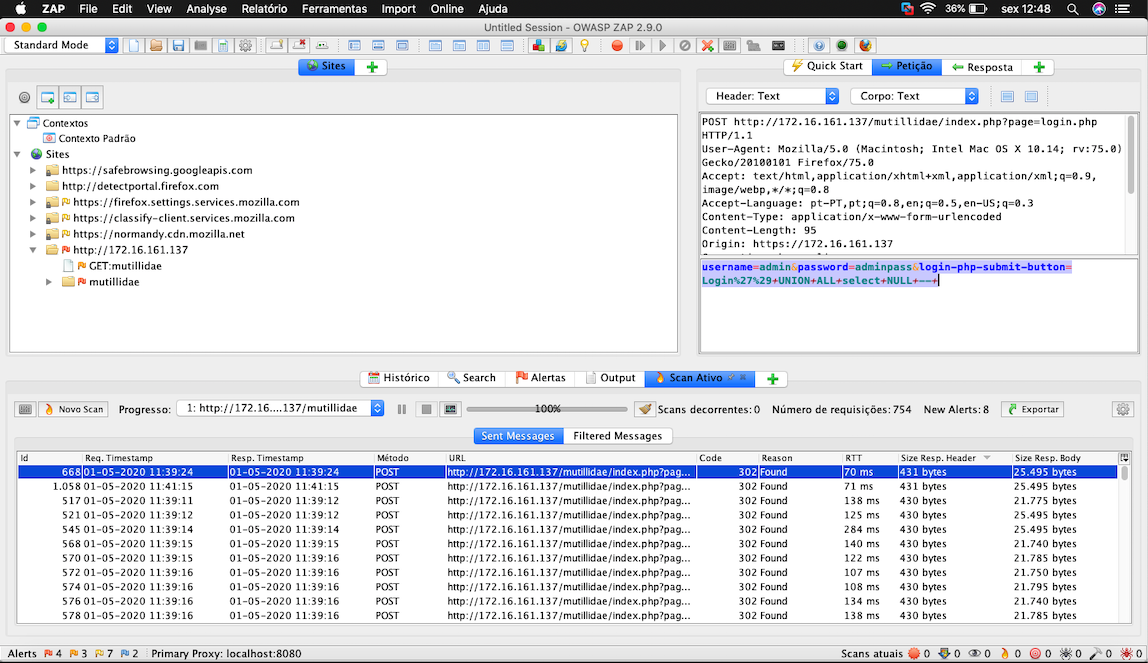
\includegraphics[scale = 0.31]{fig45.png}

  \caption{Pedido de autenticação do utilizador}

\end{figure}



Este ataque consiste portanto, em tentar alterar os campos enviados pelo utilizador para realizar este ataque.\newline
Neste caso, vamos usar o Fuzzer para modificar o campo do username com as opções XSS: URI Cross Site Scripting, XSS Style injection e XSS XML injection\footnote[1]{ Note-se que são apenas algumas opções, todas as opções apresentadas pelo ZAP são válidas.}.
\begin{figure}[H]

  \centering

  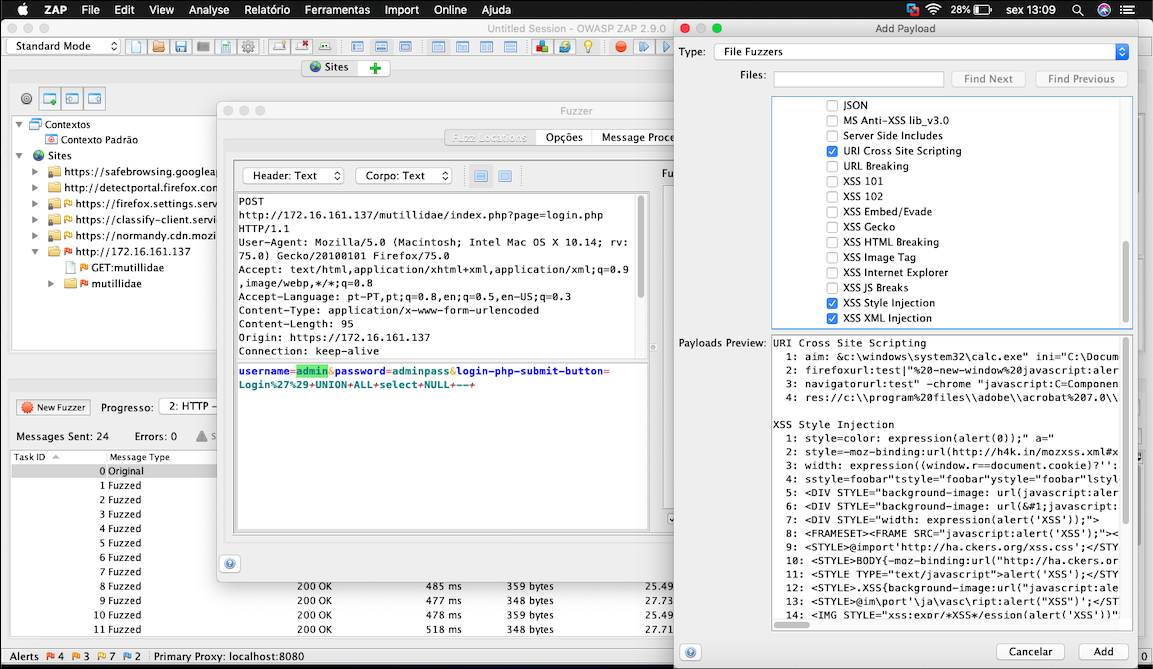
\includegraphics[scale = 0.31]{fig46.png}

  \caption{Opções de configuração do Fuzzer}

\end{figure}


 Se observarmos agora os resultados do ZAP vemos que Aparecem alguns simbolos amarelos como a nota reflected ao lado. Estes são os ataques que foram bem sucedidos na injeção de código malicioso no campo do username.

\begin{figure}[H]

  \centering

  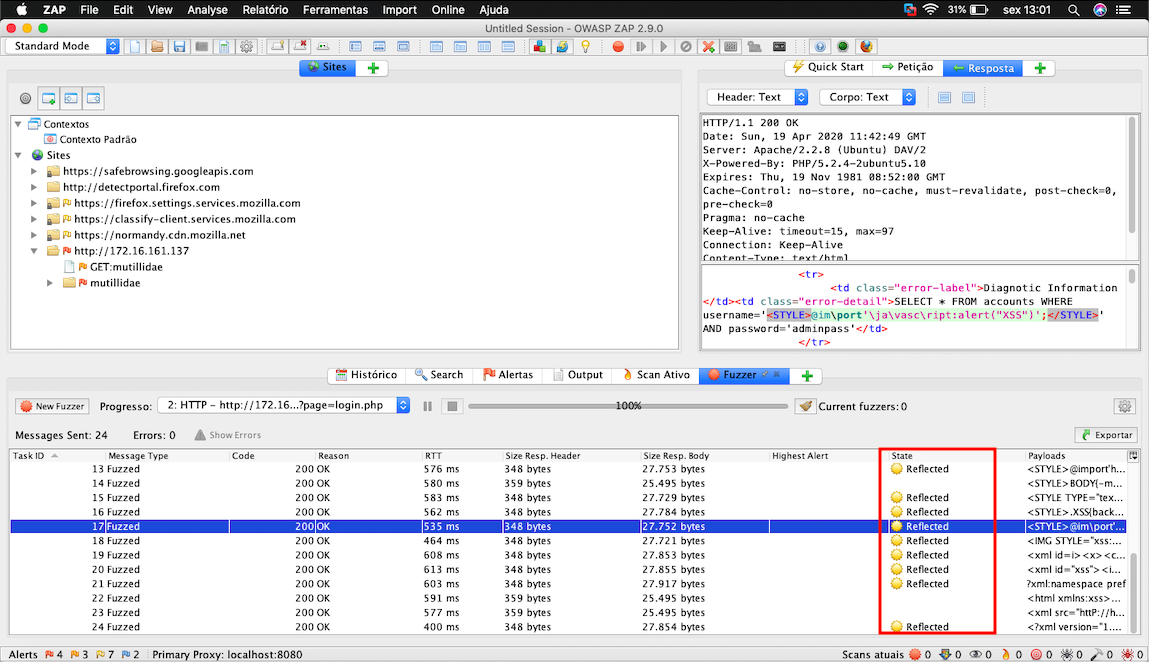
\includegraphics[scale = 0.31]{fig47.png}

  \caption{Resultados de injeção de código no campo username}

\end{figure}

Vamos então verificar o resultado no lado do utilizador caso trocassemos o campo username por um dos payloads possiveis que foram redirecionados. Neste caso para melhor visualização vamos usar o seguinte código: \textit{<script>alert('XSS');</script>}

\begin{figure}[H]

  \centering

  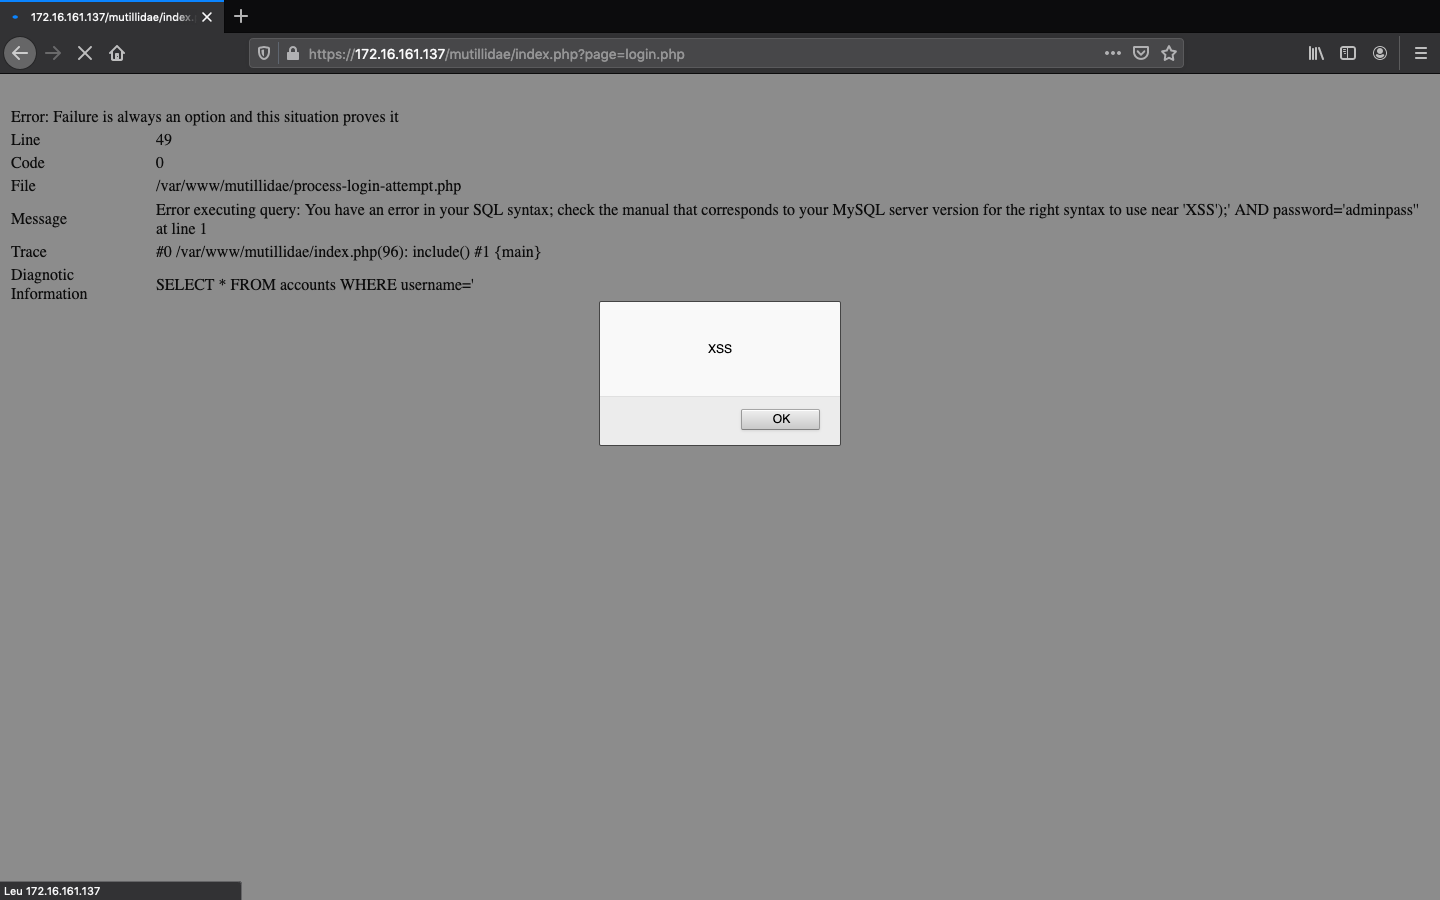
\includegraphics[scale = 0.31]{fig48.png}

  \caption{Teste de utilização de um dos payloads}

\end{figure}

%###################################### HIDDEN FILES ############################################





\subsubsection{Obter ficheiros escondidos no Servidor}

Neste ataque nós pretendemos descobrir ficheiros escondidos no servidor do site. Para isso podemos utilizar a opção "force browse directory (and children)". Nós utilizamos esta opção uma vez que a opção "force browse directory" não mostra tudo o que encontra.
\begin{figure}[H]

  \centering

  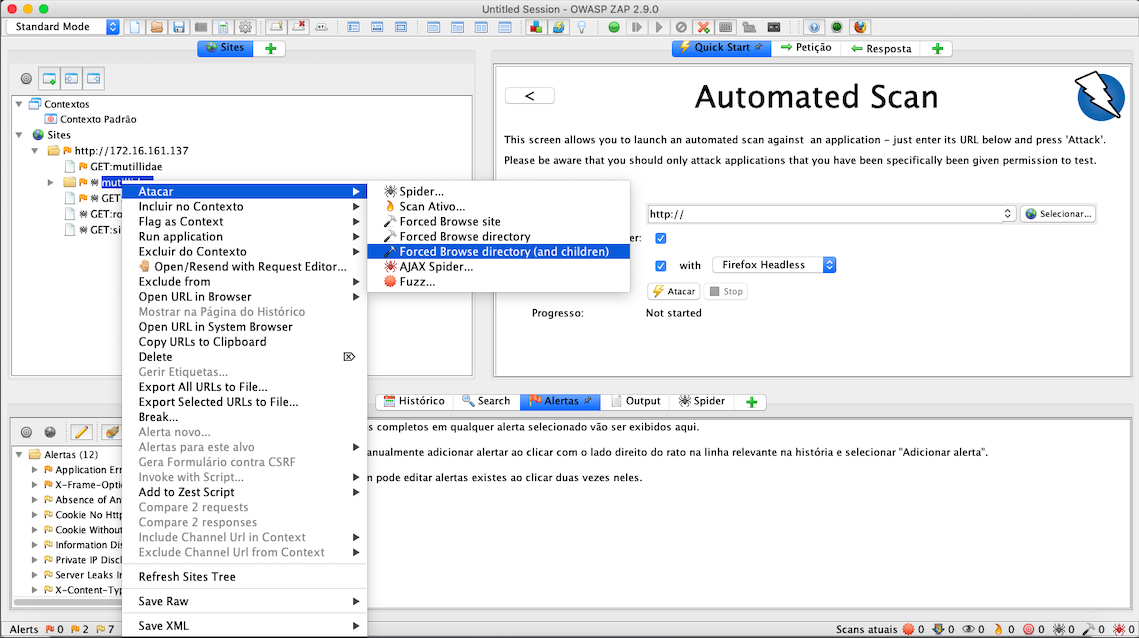
\includegraphics[scale = 0.31]{fig13.png}

  \caption{Procedimento de escolha de browse directory}

\end{figure}

É então aberta uma janela como se vê na figura seguinte. Onde selecionamos a lista que vem por defeito com o ZAP que este usará como base para uma estratégia "brute force" onde tentará encontrar os ficheros escondidos listando-os. Em baixo podemos ver o resultado da procura.
\begin{figure}[H]

  \centering

  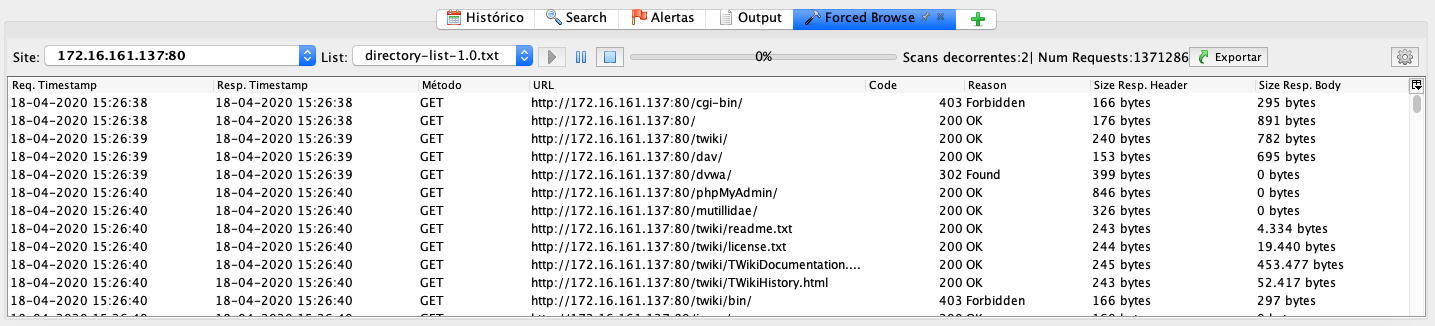
\includegraphics[scale = 0.31]{fig14.png}

  \caption{Resultados da procura}

\end{figure}

Os resultados encontrados são listados como se pode ver na figura assim com vários código associados:

-200  Ok
-403  Forbiden
-302  Found/Moved
-400  Bad Request
-500  Internal Server Error


É no entanto mais facil procurar na janela associada aos pedidos "Get" por palavras chave tais como password ou node como se pode verificar na seguinte figura e posteriormente inspecionar o conteúdo encontrado abrindo uma janela no firefox através do ZAP ou lendo o endereço do pedido get feito e inserindo o url diretamente no firefox obtendo, neste caso, uma lista de usernames e as respetivas passwords.

\begin{figure}[H]

  \centering

  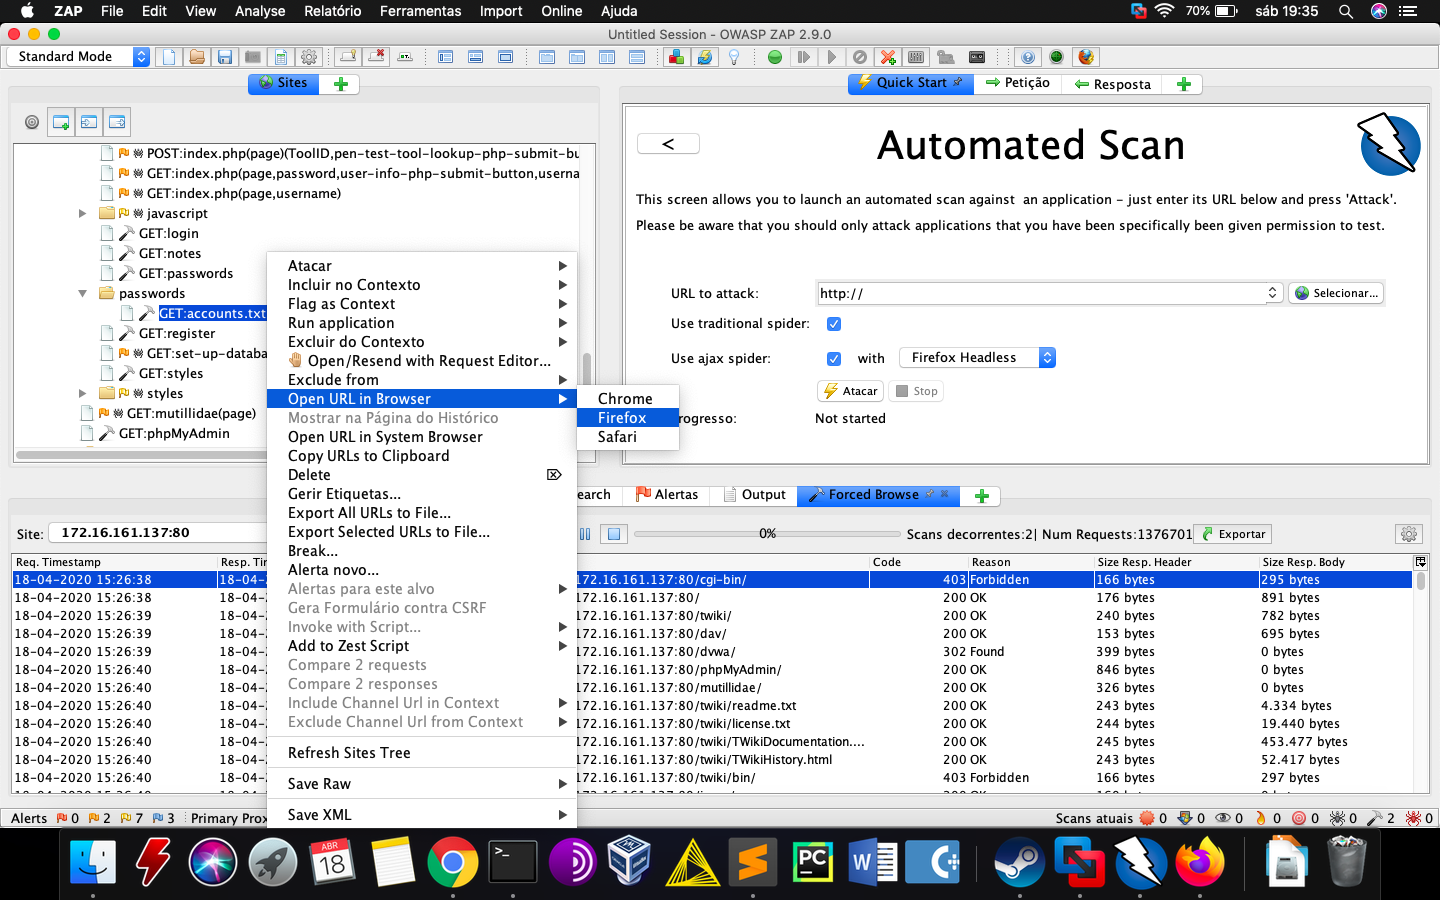
\includegraphics[scale = 0.31]{fig15_1.png}

  \caption{Abertura do URL proibido através do ZAP}

\end{figure}
\begin{figure}[H]

  \centering

  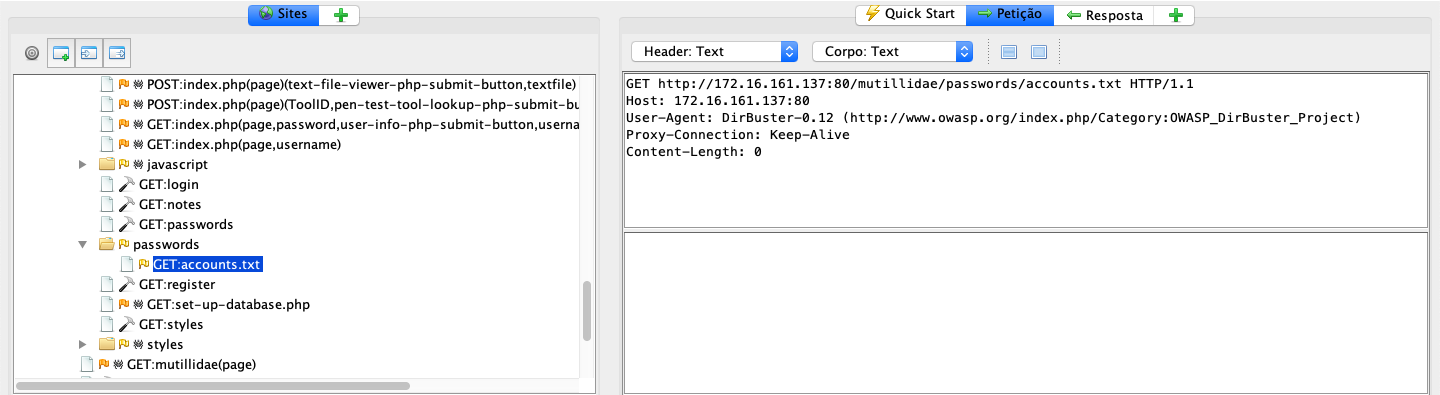
\includegraphics[scale = 0.31]{fig15_2.png}

  \caption{Pedido com o URL proibido}

\end{figure}
\begin{figure}[H]

  \centering

  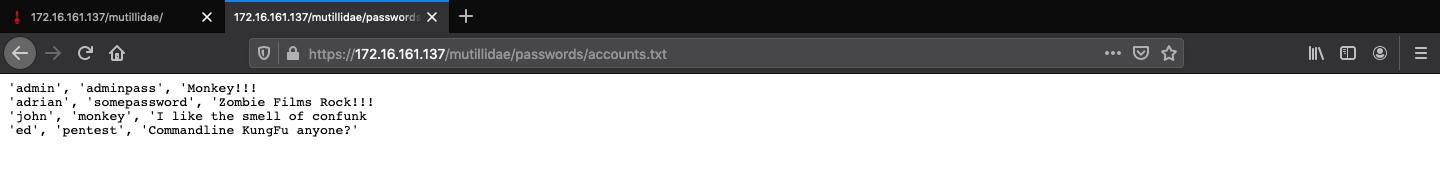
\includegraphics[scale = 0.31]{fig16.png}

  \caption{Resultado da abertura do URL desprotegido}

\end{figure}



%
% ---- Bibliography ----
%
% BibTeX users should specify bibliography style 'splncs04'.
% References will then be sorted and formatted in the correct style.
%
% \bibliographystyle{splncs04}
% \bibliography{mybibliography}
%
\begin{thebibliography}{8}
 \bibitem{ref_url1} 

\end{thebibliography}
\end{document}